\documentclass[11pt]{article}
% Shared preamble of the Korean reading editions of manuscripts A and B (XeLaTeX).
% Each main.tex loads it with % Shared preamble of the Korean reading editions of manuscripts A and B (XeLaTeX).
% Each main.tex loads it with % Shared preamble of the Korean reading editions of manuscripts A and B (XeLaTeX).
% Each main.tex loads it with \input{../common/preamble} after \documentclass[11pt]{article}.

\usepackage[a4paper,top=24mm,bottom=26mm,left=25mm,right=25mm,headheight=14pt]{geometry}

% Fonts: Latin in Times/Arial; Hangul in KoPubWorld (with a real bold) where installed,
% then Noto CJK KR, then the Batang and Malgun Gothic that ship with Windows.
\usepackage{fontspec}
\IfFontExistsTF{Times New Roman}{\setmainfont{Times New Roman}}{\setmainfont{TeX Gyre Termes}}
\IfFontExistsTF{Arial}{\setsansfont{Arial}[Scale=0.95]}{\setsansfont{TeX Gyre Heros}[Scale=0.95]}
\IfFontExistsTF{Consolas}{\setmonofont{Consolas}[Scale=0.9]}{}
\usepackage{kotex}
\IfFontExistsTF{KoPubWorldBatang Medium}{%
  \setmainhangulfont{KoPubWorldBatang Medium}[BoldFont={KoPubWorldBatang Bold},AutoFakeSlant=0.15]%
}{\IfFontExistsTF{Noto Serif CJK KR}{%
  \setmainhangulfont{Noto Serif CJK KR}[AutoFakeSlant=0.15]%
}{\setmainhangulfont{Batang}[AutoFakeSlant=0.15]}}
\IfFontExistsTF{KoPubWorldDotum Medium}{%
  \setsanshangulfont{KoPubWorldDotum Medium}[BoldFont={KoPubWorldDotum Bold},AutoFakeSlant=0.15]%
}{\IfFontExistsTF{Noto Sans CJK KR}{%
  \setsanshangulfont{Noto Sans CJK KR}[AutoFakeSlant=0.15]%
}{\setsanshangulfont{Malgun Gothic}[AutoFakeSlant=0.15]}}
\setmonohangulfont{Malgun Gothic}

\linespread{1.3}
\setlength{\parindent}{0pt}
\setlength{\parskip}{0.6em plus 0.2em minus 0.1em}
\setlength{\emergencystretch}{2em}
\raggedbottom

\usepackage{amsmath,amssymb}
\usepackage{array,booktabs,tabularx,multirow}
\usepackage{graphicx}
\usepackage[table]{xcolor}
\usepackage{tikz}
\usetikzlibrary{arrows.meta,positioning,calc}
\usepackage[most]{tcolorbox}
\usepackage{enumitem}
\setlist{itemsep=0.3em,topsep=0.2em,parsep=0.2em,leftmargin=1.7em}
\usepackage[font=small,labelfont={bf,sf},labelsep=period,justification=raggedright,
  singlelinecheck=false,skip=5pt]{caption}

\usepackage{titlesec}
\titleformat{\section}{\sffamily\Large\bfseries}{\thesection}{0.6em}{}
\titleformat{\subsection}{\sffamily\large\bfseries}{\thesubsection}{0.6em}{}
\titleformat{\subsubsection}{\sffamily\normalsize\bfseries}{\thesubsubsection}{0.6em}{}
\titleformat{\paragraph}[runin]{\sffamily\normalsize\bfseries}{}{0pt}{}
\titlespacing*{\section}{0pt}{1.4em}{0.5em}
\titlespacing*{\subsection}{0pt}{1.1em}{0.4em}
\titlespacing*{\subsubsection}{0pt}{0.9em}{0.3em}
\titlespacing*{\paragraph}{0pt}{0.6em}{0.6em}

\usepackage{fancyhdr}
\pagestyle{fancy}
\fancyhf{}
\renewcommand{\headrulewidth}{0.4pt}
\fancyhead[L]{\small\sffamily\ShortTitle}
\fancyhead[R]{\small\sffamily 쉬운 한국어 해설판}
\fancyfoot[C]{\small\thepage}
\newcommand{\ShortTitle}{}

\usepackage{longtable}
\usepackage{cite}
\PassOptionsToPackage{hyphens}{url}
\usepackage[hidelinks]{hyperref}
\urlstyle{same}

\renewcommand{\figurename}{그림}
\renewcommand{\tablename}{표}
\renewcommand{\refname}{참고문헌}
\renewcommand{\contentsname}{차례}

% Boxes. yoji: the gist of a section; puri: an explanation for the reader.
% Neither box is part of the English manuscript; the text outside the boxes is.
\newtcolorbox{yoji}{enhanced,breakable,colback=black!5,colframe=black!5,boxrule=0pt,arc=0pt,
  borderline west={2.5pt}{0pt}{black!50},left=9pt,right=8pt,top=5pt,bottom=5pt,
  before skip=0.5em,after skip=0.9em,fontupper=\small,
  before upper={\textsf{\textbf{요점}}\quad}}
\newtcolorbox{puri}[1][쉽게 풀면]{enhanced,breakable,colback=blue!3,colframe=blue!35!black!45,
  boxrule=0.5pt,arc=1.5pt,left=8pt,right=8pt,top=4pt,bottom=5pt,before skip=0.7em,after skip=0.9em,
  fontupper=\small,title={#1},fonttitle=\sffamily\bfseries\small,coltitle=black!85,
  colbacktitle=blue!9,toptitle=1pt,bottomtitle=1pt}

% Title block: \KoTitle{Korean title}{English title}{authors}{venue and source}
\newcommand{\KoTitle}[4]{%
  \thispagestyle{plain}%
  {\raggedright
  {\sffamily\bfseries\LARGE #1\par}\vspace{0.7em}
  {\large #2\par}\vspace{0.9em}
  {\small #3\par}\vspace{0.3em}
  {\small\color{black!70}#4\par}}
  \vspace{0.6em}\hrule\vspace{0.4em}}

% Numbers written only to illustrate (check_numbers.py skips what this wraps).
\newcommand{\ill}[1]{#1}
\newcommand{\dt}{\Delta\tau}
\newcommand{\Tobs}{T_{\mathrm{obs}}}
% A table cell that wraps.
\newcolumntype{L}[1]{>{\raggedright\arraybackslash}p{#1}}
\newcolumntype{Y}{>{\raggedright\arraybackslash}X}
 after \documentclass[11pt]{article}.

\usepackage[a4paper,top=24mm,bottom=26mm,left=25mm,right=25mm,headheight=14pt]{geometry}

% Fonts: Latin in Times/Arial; Hangul in KoPubWorld (with a real bold) where installed,
% then Noto CJK KR, then the Batang and Malgun Gothic that ship with Windows.
\usepackage{fontspec}
\IfFontExistsTF{Times New Roman}{\setmainfont{Times New Roman}}{\setmainfont{TeX Gyre Termes}}
\IfFontExistsTF{Arial}{\setsansfont{Arial}[Scale=0.95]}{\setsansfont{TeX Gyre Heros}[Scale=0.95]}
\IfFontExistsTF{Consolas}{\setmonofont{Consolas}[Scale=0.9]}{}
\usepackage{kotex}
\IfFontExistsTF{KoPubWorldBatang Medium}{%
  \setmainhangulfont{KoPubWorldBatang Medium}[BoldFont={KoPubWorldBatang Bold},AutoFakeSlant=0.15]%
}{\IfFontExistsTF{Noto Serif CJK KR}{%
  \setmainhangulfont{Noto Serif CJK KR}[AutoFakeSlant=0.15]%
}{\setmainhangulfont{Batang}[AutoFakeSlant=0.15]}}
\IfFontExistsTF{KoPubWorldDotum Medium}{%
  \setsanshangulfont{KoPubWorldDotum Medium}[BoldFont={KoPubWorldDotum Bold},AutoFakeSlant=0.15]%
}{\IfFontExistsTF{Noto Sans CJK KR}{%
  \setsanshangulfont{Noto Sans CJK KR}[AutoFakeSlant=0.15]%
}{\setsanshangulfont{Malgun Gothic}[AutoFakeSlant=0.15]}}
\setmonohangulfont{Malgun Gothic}

\linespread{1.3}
\setlength{\parindent}{0pt}
\setlength{\parskip}{0.6em plus 0.2em minus 0.1em}
\setlength{\emergencystretch}{2em}
\raggedbottom

\usepackage{amsmath,amssymb}
\usepackage{array,booktabs,tabularx,multirow}
\usepackage{graphicx}
\usepackage[table]{xcolor}
\usepackage{tikz}
\usetikzlibrary{arrows.meta,positioning,calc}
\usepackage[most]{tcolorbox}
\usepackage{enumitem}
\setlist{itemsep=0.3em,topsep=0.2em,parsep=0.2em,leftmargin=1.7em}
\usepackage[font=small,labelfont={bf,sf},labelsep=period,justification=raggedright,
  singlelinecheck=false,skip=5pt]{caption}

\usepackage{titlesec}
\titleformat{\section}{\sffamily\Large\bfseries}{\thesection}{0.6em}{}
\titleformat{\subsection}{\sffamily\large\bfseries}{\thesubsection}{0.6em}{}
\titleformat{\subsubsection}{\sffamily\normalsize\bfseries}{\thesubsubsection}{0.6em}{}
\titleformat{\paragraph}[runin]{\sffamily\normalsize\bfseries}{}{0pt}{}
\titlespacing*{\section}{0pt}{1.4em}{0.5em}
\titlespacing*{\subsection}{0pt}{1.1em}{0.4em}
\titlespacing*{\subsubsection}{0pt}{0.9em}{0.3em}
\titlespacing*{\paragraph}{0pt}{0.6em}{0.6em}

\usepackage{fancyhdr}
\pagestyle{fancy}
\fancyhf{}
\renewcommand{\headrulewidth}{0.4pt}
\fancyhead[L]{\small\sffamily\ShortTitle}
\fancyhead[R]{\small\sffamily 쉬운 한국어 해설판}
\fancyfoot[C]{\small\thepage}
\newcommand{\ShortTitle}{}

\usepackage{longtable}
\usepackage{cite}
\PassOptionsToPackage{hyphens}{url}
\usepackage[hidelinks]{hyperref}
\urlstyle{same}

\renewcommand{\figurename}{그림}
\renewcommand{\tablename}{표}
\renewcommand{\refname}{참고문헌}
\renewcommand{\contentsname}{차례}

% Boxes. yoji: the gist of a section; puri: an explanation for the reader.
% Neither box is part of the English manuscript; the text outside the boxes is.
\newtcolorbox{yoji}{enhanced,breakable,colback=black!5,colframe=black!5,boxrule=0pt,arc=0pt,
  borderline west={2.5pt}{0pt}{black!50},left=9pt,right=8pt,top=5pt,bottom=5pt,
  before skip=0.5em,after skip=0.9em,fontupper=\small,
  before upper={\textsf{\textbf{요점}}\quad}}
\newtcolorbox{puri}[1][쉽게 풀면]{enhanced,breakable,colback=blue!3,colframe=blue!35!black!45,
  boxrule=0.5pt,arc=1.5pt,left=8pt,right=8pt,top=4pt,bottom=5pt,before skip=0.7em,after skip=0.9em,
  fontupper=\small,title={#1},fonttitle=\sffamily\bfseries\small,coltitle=black!85,
  colbacktitle=blue!9,toptitle=1pt,bottomtitle=1pt}

% Title block: \KoTitle{Korean title}{English title}{authors}{venue and source}
\newcommand{\KoTitle}[4]{%
  \thispagestyle{plain}%
  {\raggedright
  {\sffamily\bfseries\LARGE #1\par}\vspace{0.7em}
  {\large #2\par}\vspace{0.9em}
  {\small #3\par}\vspace{0.3em}
  {\small\color{black!70}#4\par}}
  \vspace{0.6em}\hrule\vspace{0.4em}}

% Numbers written only to illustrate (check_numbers.py skips what this wraps).
\newcommand{\ill}[1]{#1}
\newcommand{\dt}{\Delta\tau}
\newcommand{\Tobs}{T_{\mathrm{obs}}}
% A table cell that wraps.
\newcolumntype{L}[1]{>{\raggedright\arraybackslash}p{#1}}
\newcolumntype{Y}{>{\raggedright\arraybackslash}X}
 after \documentclass[11pt]{article}.

\usepackage[a4paper,top=24mm,bottom=26mm,left=25mm,right=25mm,headheight=14pt]{geometry}

% Fonts: Latin in Times/Arial; Hangul in KoPubWorld (with a real bold) where installed,
% then Noto CJK KR, then the Batang and Malgun Gothic that ship with Windows.
\usepackage{fontspec}
\IfFontExistsTF{Times New Roman}{\setmainfont{Times New Roman}}{\setmainfont{TeX Gyre Termes}}
\IfFontExistsTF{Arial}{\setsansfont{Arial}[Scale=0.95]}{\setsansfont{TeX Gyre Heros}[Scale=0.95]}
\IfFontExistsTF{Consolas}{\setmonofont{Consolas}[Scale=0.9]}{}
\usepackage{kotex}
\IfFontExistsTF{KoPubWorldBatang Medium}{%
  \setmainhangulfont{KoPubWorldBatang Medium}[BoldFont={KoPubWorldBatang Bold},AutoFakeSlant=0.15]%
}{\IfFontExistsTF{Noto Serif CJK KR}{%
  \setmainhangulfont{Noto Serif CJK KR}[AutoFakeSlant=0.15]%
}{\setmainhangulfont{Batang}[AutoFakeSlant=0.15]}}
\IfFontExistsTF{KoPubWorldDotum Medium}{%
  \setsanshangulfont{KoPubWorldDotum Medium}[BoldFont={KoPubWorldDotum Bold},AutoFakeSlant=0.15]%
}{\IfFontExistsTF{Noto Sans CJK KR}{%
  \setsanshangulfont{Noto Sans CJK KR}[AutoFakeSlant=0.15]%
}{\setsanshangulfont{Malgun Gothic}[AutoFakeSlant=0.15]}}
\setmonohangulfont{Malgun Gothic}

\linespread{1.3}
\setlength{\parindent}{0pt}
\setlength{\parskip}{0.6em plus 0.2em minus 0.1em}
\setlength{\emergencystretch}{2em}
\raggedbottom

\usepackage{amsmath,amssymb}
\usepackage{array,booktabs,tabularx,multirow}
\usepackage{graphicx}
\usepackage[table]{xcolor}
\usepackage{tikz}
\usetikzlibrary{arrows.meta,positioning,calc}
\usepackage[most]{tcolorbox}
\usepackage{enumitem}
\setlist{itemsep=0.3em,topsep=0.2em,parsep=0.2em,leftmargin=1.7em}
\usepackage[font=small,labelfont={bf,sf},labelsep=period,justification=raggedright,
  singlelinecheck=false,skip=5pt]{caption}

\usepackage{titlesec}
\titleformat{\section}{\sffamily\Large\bfseries}{\thesection}{0.6em}{}
\titleformat{\subsection}{\sffamily\large\bfseries}{\thesubsection}{0.6em}{}
\titleformat{\subsubsection}{\sffamily\normalsize\bfseries}{\thesubsubsection}{0.6em}{}
\titleformat{\paragraph}[runin]{\sffamily\normalsize\bfseries}{}{0pt}{}
\titlespacing*{\section}{0pt}{1.4em}{0.5em}
\titlespacing*{\subsection}{0pt}{1.1em}{0.4em}
\titlespacing*{\subsubsection}{0pt}{0.9em}{0.3em}
\titlespacing*{\paragraph}{0pt}{0.6em}{0.6em}

\usepackage{fancyhdr}
\pagestyle{fancy}
\fancyhf{}
\renewcommand{\headrulewidth}{0.4pt}
\fancyhead[L]{\small\sffamily\ShortTitle}
\fancyhead[R]{\small\sffamily 쉬운 한국어 해설판}
\fancyfoot[C]{\small\thepage}
\newcommand{\ShortTitle}{}

\usepackage{longtable}
\usepackage{cite}
\PassOptionsToPackage{hyphens}{url}
\usepackage[hidelinks]{hyperref}
\urlstyle{same}

\renewcommand{\figurename}{그림}
\renewcommand{\tablename}{표}
\renewcommand{\refname}{참고문헌}
\renewcommand{\contentsname}{차례}

% Boxes. yoji: the gist of a section; puri: an explanation for the reader.
% Neither box is part of the English manuscript; the text outside the boxes is.
\newtcolorbox{yoji}{enhanced,breakable,colback=black!5,colframe=black!5,boxrule=0pt,arc=0pt,
  borderline west={2.5pt}{0pt}{black!50},left=9pt,right=8pt,top=5pt,bottom=5pt,
  before skip=0.5em,after skip=0.9em,fontupper=\small,
  before upper={\textsf{\textbf{요점}}\quad}}
\newtcolorbox{puri}[1][쉽게 풀면]{enhanced,breakable,colback=blue!3,colframe=blue!35!black!45,
  boxrule=0.5pt,arc=1.5pt,left=8pt,right=8pt,top=4pt,bottom=5pt,before skip=0.7em,after skip=0.9em,
  fontupper=\small,title={#1},fonttitle=\sffamily\bfseries\small,coltitle=black!85,
  colbacktitle=blue!9,toptitle=1pt,bottomtitle=1pt}

% Title block: \KoTitle{Korean title}{English title}{authors}{venue and source}
\newcommand{\KoTitle}[4]{%
  \thispagestyle{plain}%
  {\raggedright
  {\sffamily\bfseries\LARGE #1\par}\vspace{0.7em}
  {\large #2\par}\vspace{0.9em}
  {\small #3\par}\vspace{0.3em}
  {\small\color{black!70}#4\par}}
  \vspace{0.6em}\hrule\vspace{0.4em}}

% Numbers written only to illustrate (check_numbers.py skips what this wraps).
\newcommand{\ill}[1]{#1}
\newcommand{\dt}{\Delta\tau}
\newcommand{\Tobs}{T_{\mathrm{obs}}}
% A table cell that wraps.
\newcolumntype{L}[1]{>{\raggedright\arraybackslash}p{#1}}
\newcolumntype{Y}{>{\raggedright\arraybackslash}X}

\renewcommand{\ShortTitle}{원고 A · PLOS ONE}

\begin{document}

\KoTitle{허락 화살표인가, 송금 화살표인가?\\[0.25em]\Large 스마트 계약의 온체인 평판 점수를 기간 밖에서 원시 차수와 견주어 평가하기}
{Allowance edges or transfer edges? Evaluating on-chain smart contract reputation out of window against degree baselines}
{Taehong Kwon, Ernest Mnkandla, Donatien Koulla Moulla, David Sena Attipoe\\
School of Computing, University of South Africa}
{PLOS ONE에 낼 원고 A(Research Article)의 쉬운 한국어 해설판 · 영문 원고: 원고 저장소 \texttt{07391e9}의 \texttt{manuscripts/A-plos-one}}

\section*{이 글을 읽는 법}

\begin{itemize}
\item 영문 원고 A를 쉬운 한국어로 풀어 쓴 글이에요. 절의 순서는 영문 원고와 같지만, 문장을 하나하나 옮긴 번역은 아니에요.
\item 회색 \textsf{\textbf{요점}} 상자는 그 절의 핵심이고, 파란 상자는 낯선 개념과 표 읽는 법을 풀어 줘요. 두 상자는 영문 원고에 없어요. 상자 밖 본문이 영문 원고의 내용이에요.
\item 수와 구간은 모두 영문 원고와 같아요. “0.560 [0.548, 0.571]”은 점 추정값 0.560과 그 95\% 신뢰구간이에요. 따로 97.5\%라고 적지 않은 구간은 모두 95\% 구간이에요. 두 점수의 차이는 그 구간이 0을 포함하지 않을 때만 “차이가 있다”고 말해요.
\end{itemize}

{\small\setcounter{tocdepth}{1}\tableofcontents}

%======================================================================
\section*{한눈에 보기: 초록}
\addcontentsline{toc}{section}{한눈에 보기: 초록}

\paragraph{무엇을 묻나요?}
디파이(DeFi, 탈중앙 금융) 계약을 쓰기 전에, 토큰 주인은 ERC-20 허락에 서명해요. 그 계약이 자기 토큰을 옮겨도 된다고 허락하는 거예요. 그래프로 만든 평판 점수가 이 결정을 도울 수 있어요. 그런데 이미 있는 방법인 AWP(적응형 가중 페이지랭크)는 송금 화살표를 따라 걸어요. 송금은 돈을 치른 기록이지, 무엇을 허락한 기록이 아니에요. 그래서 이 원고는 허락 화살표가 무엇을 더해 주는지 물어요.

\paragraph{무엇을 비교했나요?}
아비트럼 원(Arbitrum One)의 공개 로그로, 서로 다른 주인 셋 이상에게 허락을 받은 계약 6,483개를 점수 매겼어요. 비교한 점수는 넷이에요.
\begin{itemize}
\item 엔도스랭크(EndorseRank): 마지막 허락 위를 걷는 페이지랭크.
\item AWP: 송금 위를 걷는 페이지랭크.
\item 두 걷기가 각각 매끄럽게 다듬는 원시 차수 두 가지: 받은 허락 수(허락한 서로 다른 주인 수)와 송금 입차수(송금을 보내온 서로 다른 주소 수).
\end{itemize}
금액은 다섯 토큰의 달러 값으로 재고, 점수는 동결 직전 12개월의 사건으로 만들었어요. 이 세 가지(달러 금액, 다섯 토큰, 12개월 점수 기간)는 원래 단위로 미리 정해 둔 분석이 다 끝난 뒤에 정했어요. 원고는 이 수정 분석을 보고하고, 미리 정한 규칙은 재분석으로 적용해요.

\paragraph{무엇을 찾았나요?}
\begin{enumerate}
\item \textbf{같은 기간: 점수는 자기 화살표와 가장 잘 맞아요.} 엔도스랭크는 허락으로 만든 점검과 켄달의 $\tau$ 0.560 [0.548, 0.571], AWP는 송금으로 만든 점검과 0.736 [0.728, 0.744]만큼 맞았어요.
\item \textbf{기간 밖: 어느 걷기도 원시 차수를 넘지 못했어요.} 석 달짜리 두 창(W0, W1) 앞에서 점수를 동결하고, 그 뒤에 생긴 일로 채점했어요. 계약마다 나중에 새로 송금해 온 주소의 수(새 송금자)를 세면, AWP는 이 수를 송금 입차수만큼 잘 줄 세우지 못했어요($\dt$ −0.038 [−0.043, −0.032]와 −0.041 [−0.047, −0.034]). 엔도스랭크도 나중에 새로 허락해 준 주인의 수(새 허락 쌍)를 허락한 주인 수만큼 잘 줄 세우지 못했어요(−0.090 [−0.100, −0.079]와 −0.082 [−0.090, −0.073]). 엔도스랭크는 활동 재시작을 써도 마찬가지였어요. 이 비교들은 라벨을 안 뒤에 고른 것이에요.
\item \textbf{엔도스랭크가 실제로 계산하는 것.} 주인들이 다른 주소에게서 허락을 받지 않는 스펜더에서, 엔도스랭크는 무게를 다시 단 허락 수예요.
\item \textbf{어느 그래프에도 없는 결과.} GMX V2에서 거래하는 계약 70개의 나중 청산 없이 닫은 비율에서, 허락한 주인 수가 송금 수보다 트레이더를 더 잘 줄 세웠어요($\dt$ +0.141, 97.5\% 구간 [0.026, 0.256]). 이 재분석에서는 미리 정한 규칙을 만족하지만, 미리 정한 분석에서는 만족하지 않았어요. 두 페이지랭크의 쌍은 판가름 나지 않았어요(+0.023, 97.5\% 구간 [−0.071, 0.127]).
\item \textbf{계산 비용.} AWP의 그래프는 화살표가 2.21배 많았고, 같은 풀이 프로그램으로 푸는 데 3.21배 오래 걸렸어요.
\end{enumerate}

\paragraph{무엇을 조심해야 하나요?}
수정 분석의 판정은 등록한 시험의 결과가 아니라 재분석이에요. 걷기와 원시 차수의 비교는 모두 라벨을 안 뒤에 골랐어요. 트레이더 표본은 70–87개로 작아요. 그리고 이 원고는 인과를 주장하지 않아요.

\begin{puri}[한 문장으로 줄이면]
허락으로 만든 점수는 나중의 새 허락을, 송금으로 만든 점수는 나중의 새 송금자를 잘 맞혀요. 하지만 수정 분석에서는, 걸어서 퍼뜨린 페이지랭크가 같은 종류의 나중 화살표를 그 화살표를 그냥 센 수(원시 차수)만큼 잘 줄 세운 적이 두 창 어디에서도 없었어요(라벨을 안 뒤에 한 비교예요). 등록 분석에서는 AWP와 활동 재시작 엔도스랭크가 자기 수를 넘었어요.
\end{puri}

%======================================================================
\section*{먼저 알아 둘 말}
\addcontentsline{toc}{section}{먼저 알아 둘 말}

{\small
\renewcommand{\arraystretch}{1.25}
\begin{longtable}{@{}L{3.6cm}L{11.9cm}@{}}
\toprule
말 & 뜻 \\
\midrule
\endhead
스마트 계약(계약) & 블록체인 위에서 저절로 실행되는 프로그램이에요. 이 원고가 점수를 매기는 대상은 계약뿐이에요. \\
외부 소유 계정(EOA) & 개인 키로 움직이는 계정이에요. 그래프에는 주인, 보낸 쪽, 받는 쪽으로만 나오고, 점수를 받거나 보고되지 않아요. \\
허락(allowance) & 토큰 주인이 어떤 계약에게 “내 토큰을 이만큼까지 옮겨도 된다”고 허락한 기록이에요. \texttt{approve}를 부르거나 \texttt{permit}에 서명해서 만들어요. \\
주인, 스펜더 & 허락을 해 주는 쪽과, 허락을 받아 대신 쓰는 쪽(계약)이에요. \\
마지막 허락 & 같은 주인, 스펜더, 토큰의 가장 최근 허락이에요. 새 허락은 옛 허락을 덮어쓰고, 0으로 하면 허락이 없어져요. \\
송금(transfer) & 토큰이 한 주소에서 다른 주소로 옮겨진 기록이에요. \\
허락 그래프, 송금 그래프 & 점(주소)과 화살표로 이은 그림이에요. 허락 그래프의 화살표는 주인 → 스펜더, 송금 그래프의 화살표는 보낸 쪽 → 받는 쪽이에요. \\
원시 차수 & 화살표를 그냥 센 수예요. 받은 허락 수(그 계약에 양수의 마지막 허락을 둔 서로 다른 주인 수)와 송금 입차수(그 계약에 송금한 적 있는 서로 다른 주소 수)를 써요. \\
허락 수, 송금 수 & 받은 허락 수와 송금 입차수를 줄여 부른 말이에요. 송금 건수가 아니라 서로 다른 주소의 수예요. \\
페이지랭크 & 화살표를 따라 무작위로 걷다가, 가끔 재시작 분포에 따라 고른 점으로 건너뛰어 다시 출발할 때, 아주 오래 걸으면 각 점에 머무는 비율이에요. 이 원고는 화살표를 따라갈 확률(감쇠 계수) $d=0.85$를 써요. \\
엔도스랭크 & 마지막 허락 그래프 위의 페이지랭크예요. 화살표 무게는 AWP와 같은 식으로 달고, 모든 점에서 고르게 다시 출발해요. \\
AWP & 송금 그래프 위의 페이지랭크예요. 금액과 시간으로 화살표 무게를 달고, 최근에 송금한 주소에서 더 자주 다시 출발해요. \\
활동 재시작 & AWP처럼 활발한 주소에서 더 자주 다시 출발하는 규칙이에요. 엔도스랭크의 변형 하나가 이 규칙을 써요. \\
동결, 점수 기간 & 점수를 고정하는 시점이 동결이에요. 점수는 동결 직전 12개월(점수 기간)의 사건으로만 만들어요. \\
라벨, 라벨 기간 & 동결 뒤 석 달(라벨 기간) 동안 일어난 일로 센 값이에요. 점수가 이것을 얼마나 잘 줄 세우는지로 채점해요. \\
W0, W1 & 시험 창 두 개예요. W0은 2026년 3월 31일에 동결하고 4–6월을, W1은 2026년 6월 30일에 동결하고 7–9월을 라벨 기간으로 써요. 트레이더 비교에서는 W1이 주 창이에요. \\
켄달의 타우($\tau_b$) & 두 줄 세우기가 얼마나 같은 순서인지 나타내는 수예요. 1이면 순서가 완전히 같고, 0이면 순서의 경향이 없고, −1이면 정반대예요. 동점이 많을 때를 바로잡은 꼴($\tau_b$)을 써요. \\
$\dt$ & 두 점수의 타우 차이, $\tau(a)-\tau(b)$예요. 양수면 $a$가 라벨을 더 잘 줄 세운 거예요. \\
짝지은 부트스트랩 & 계약들을 되돌려 넣으며 다시 뽑아 같은 계산을 수백, 수천 번 되풀이해서, 값이 얼마나 흔들리는지 보는 방법이에요. 두 점수에 같은 다시 뽑기를 써서, 두 계수가 함께 흔들리는 정도(공분산)를 살린 채 차이의 구간을 구해요. \\
95\% 구간, 97.5\% 구간 & 다시 뽑은 결과의 가운데 95\%가 놓인 범위예요. 97.5\% 구간은 판정 대비 두 개(P와 Q)를 함께 볼 때 쓰는 더 넓은 구간(본페로니 구간)이에요. \\
등록 분석 & 분석 계획과 W1 등록 문서에 미리 정한 그대로 한 분석이에요. 금액은 원래 단위, 모든 ERC-20 토큰, 2023년 10월 1일부터의 모든 사건으로 점수를 만들었어요. \\
수정 분석, 재분석 & 등록 분석의 결과를 안 뒤에 정한 분석이에요. 금액은 달러, 토큰은 다섯 개, 점수는 동결 직전 12개월의 사건으로 만들어요. 등록한 규칙을 여기에 적용한 것은 재분석이라고 불러요. \\
GMX V2, 청산 & 아비트럼 원의 무기한 선물 거래소와, 담보가 손실을 감당하지 못해 포지션이 강제로 닫히는 일이에요. \\
청산 없이 닫은 비율(LFCR) & 라벨 기간에 닫은 포지션 가운데 청산이 아니었던 몫이에요. 트레이더 비교의 주 라벨이에요. \\
\bottomrule
\end{longtable}}
\addtocounter{table}{-1}% the glossary is not a numbered table

%======================================================================
\section{들어가며}

\begin{yoji}
토큰 주인은 어느 계약에 허락을 줄지 정해야 해요. 다른 주인들이 이미 어느 계약에 허락을 줬는지는 공개 장부에 남아 있어요. 이 원고는 허락 기록과 송금 기록 가운데 어느 쪽이 계약의 평판 점수로 쓸모 있는지를, 기간 밖의 자료와 원시 차수라는 기준선으로 따져요.
\end{yoji}

\subsection{허락 하나로 잔고 전체가 위험해질 수 있어요}

디파이는 대출, 거래, 자산 관리를 공개 블록체인 위의 스마트 계약으로 해요~\cite{schar2021defi,werner2022sok}. 이런 서비스는 대부분 허락에서 시작해요. 토큰 주인이 어떤 계약에게 자기 토큰의 일부를 옮겨도 된다고 허락하는 거예요. ERC-20 토큰은 이 허락을 허락(allowance) 값으로 저장해요. 주인은 \texttt{approve}를 부르거나 EIP-2612의 \texttt{permit}에 서명해서 이 값을 정해요~\cite{vogelsteller2015erc20,lundfall2020permit}.

허락은 다 쓰거나, 새 허락으로 바꾸거나, 거둘 때까지 계속 살아 있어요. 그리고 이더리움의 허락은 대부분 금액에 제한이 없는 무제한 허락이에요~\cite{wang2022unlimited}. 그래서 나쁜 계약이, 또는 정직했지만 나중에 뚫린 계약이, 주인이 허락한 토큰의 잔고를 통째로 가져갈 수 있어요. 피싱 사이트는 사용자가 바로 이런 허락에 서명하도록 이끌고~\cite{he2023txphishscope}, 그렇게 하는 도구 묶음은 서비스로 팔려요~\cite{he2025drainer}. 그래서 주인과 주인의 지갑 프로그램, 그리고 다른 계약 위에 서비스를 짓는 프로토콜은 모두 같은 질문을 안고 있어요. 어느 스펜더 계약이 허락을 받을 만한가요?

\subsection{지금은 계약을 어떻게 믿나요}

지금 스펜더 계약에 대한 믿음은 몇 가지 길로 생겨요.
\begin{itemize}
\item 대부분의 주인은 지갑이 허락 요청을 보여 줄 때 결정해요. 그런데 지갑이 허락을 보여 주고 확인하는 방식에 빈틈이 있어서, 바로 그 순간이 사기에 열려 있어요~\cite{adamczyk2025approval}.
\item 코드 분석은 계약을 그 함수로 판단해요. 예를 들어 러그 풀(돈을 모은 뒤 갑자기 빼 가는 사기)을 위해 쓴 함수를 찾아내요~\cite{lin2024crpwarner}.
\item 휴먼 패스포트(Human Passport) 같은 평판 도구는 자격 증명에 무게를 달아, 한 주소가 서로 다른 한 사람의 것인지 판단해요~\cite{humanpassportnddocs}. 이것은 키를 가진 사람에 관한 질문이라, 계약에는 바로 맞는 짝이 없어요.
\end{itemize}
이 가운데 어느 것도 다른 주인들이 이미 내린 결정의 공개 기록, 곧 많은 주인이 어느 계약에 허락을 줬는지를 쓰지 않아요.

\subsection{그래프 순위 매기기와 AWP}

그래프 순위 매기기는 이 기록을 읽는 한 가지 방법이에요. 페이지랭크는 방향이 있는 화살표를 따라, 감쇠 계수를 쓰는 무작위 걷기를 할 때 각 점에 머무는 정상 확률을 그 점의 점수로 줘요~\cite{page1999pagerank,langville2006pagerank}. 아이겐트러스트(EigenTrust)와 트러스트랭크(TrustRank)는 이 걷기를 P2P 네트워크의 신뢰와 웹 스팸에 맞게 고친 것이에요~\cite{kamvar2003eigentrust,gyongyi2004trustrank}.

계정 기반 장부에서는 지금까지 화살표가 늘 지급, 곧 송금이었어요. Do와 Do는 이더리움 거래에 페이지랭크와 호지랭크(HodgeRank)를 적용해 사회적 신용을 재요~\cite{do2023hodgerank}. Do, Do, Nguyen의 AWP(적응형 가중 페이지랭크)는 송금마다 무게를 달아요~\cite{do2023awp}.
\begin{itemize}
\item 무게는 금액이 클수록 커지지만 상한이 있어요.
\item 오래된 송금일수록 무게가 로지스틱 곡선을 따라 작아져요.
\item 걷기는 최근에 송금한 주소에서 다시 출발해요.
\end{itemize}
AWP의 저자들은 AWP를 각 주소가 받은 송금의 건수와 금액에 견줘 점검해요. 그런데 이것은 AWP의 그래프를 이루는 바로 그 송금으로 만든 통계예요.

\subsection{송금과 허락은 다른 일을 기록해요}

송금은 값이 옮겨졌다는 것만 보여 줘요. 보낸 쪽이 받는 쪽을 보증한다는 뜻은 아니에요. 라우터(거래를 중계하는 계약), 시장 조성자, 에어드롭 사냥꾼, 자전 거래자는 모두 송금을 대량으로 만들어요~\cite{cong2023washtrading,luo2025airdrop}.

허락은 다른 행동을 기록해요. 돈을 가진 쪽이 스펜더 하나를 골라, 정한 금액까지 옮겨도 된다고 허락해요. 같은 주인, 스펜더, 토큰의 새 허락은 옛 허락을 바꿔 쓰므로, 마지막 허락 하나가 둘 사이의 관계를 요약해요. 그리고 허락은 송금보다 드물어요.

하지만 허락이 꼭 믿음을 나타내지는 않아요. 거래소에서 거래하려면, 사용자는 그 라우터를 어떻게 생각하든 먼저 허락해야 해요. 피싱 계약도 정직한 계약처럼 허락을 모아요. 그래서 이 원고는 허락 화살표를 권한 부여(authorization)라고 부르고, 엔도스랭크라는 이름은 방법의 이름표로만 써요. 허락은 한 주체가 가진 여러 주소를 묶는 데 쓰인 적이 있어요~\cite{victor2020clustering}. 하지만 허락으로 계약의 순위를 매기는 평판 방법은 저자들이 아는 한 없어요.

\subsection{평가 설계의 두 가지 버릇}

어느 화살표가 계약의 평판 점수로 더 나은지는 얼마쯤 평가 설계의 문제예요. 이 분야의 두 가지 버릇이 이 질문에 답하기 어렵게 해요.

첫째, 점수를 자기 화살표로 만든 통계에 견줘 점검하는 버릇이에요. 이런 일치는 만든 방식 때문에 저절로 예상되는 일치예요. 그래서 이 일치는 점수가 재려는 생각(의도한 구성개념)과 앞뒤가 맞는지를 보여 줄 뿐, 점수가 그 밖에 무엇을 알려 주는지는 말해 주지 않아요~\cite{cronbach1955construct,messick1995validity}.

둘째, 걷기를 다른 걷기하고만 견주는 버릇이에요. 페이지랭크는 그 점의 수(들어오는 화살표 수)를 매끄럽게 다듬은 것이고, 그런 수는 이기기 어려워요. 새 화살표는 이미 화살표가 많은 점에 더 잘 붙어요~\cite{barabasi1999scaling,newman2001clustering}. 차수는 링크 예측의 표준 기준선이고~\cite{libennowell2007link}, 이더리움에서도 그래요~\cite{lin2022tracking}. 그리고 차수끼리의 상관이 약한 곳에서는 페이지랭크가 평균적으로 들어오는 화살표 수에 비례해요~\cite{fortunato2008indegree}. 그러니 퍼뜨려 만든 점수는 그 밑에 깔린 수를 이길 때만 더 드는 계산값을 해요.

\begin{puri}[“원시 차수를 이긴다”는 무슨 뜻인가요?]
페이지랭크는 화살표를 따라 점수를 여러 번 퍼뜨려요. 그러면 “나에게 허락을 준 주인 자신은 얼마나 높은 점수인가”까지 점수에 들어가요. 그 대신 계산이 비싸요. 화살표를 그냥 센 수(원시 차수)가 나중 일을 똑같이, 또는 더 잘 맞힌다면 퍼뜨리는 계산은 값을 하지 못해요. 그래서 이 원고는 각 페이지랭크를 그 페이지랭크가 다듬는 원시 차수와 직접 견줘요. 엔도스랭크는 받은 허락 수와, AWP는 송금 입차수와 견줘요.
\end{puri}

\subsection{이 원고가 하는 일}

이 원고는 아비트럼 원의 스마트 계약을 두고, 두 화살표 종류를 평판 점수로 견줘요. 같은 계약들에 다음 점수를 매겨요.
\begin{itemize}
\item 엔도스랭크: 마지막 허락 위의 페이지랭크예요. AWP의 화살표 무게를 쓰고, 고르게 다시 출발해요.
\item AWP.
\item 들어오는 원시 차수 두 가지.
\end{itemize}
모든 점수를 석 달짜리 라벨 기간 두 개 앞에서 동결하고, 그 뒤에 일어난 일로 각 점수를 시험해요. 점수를 받는 주소는 모두 계약 코드를 가진 주소예요. 외부 소유 계정은 주인, 보낸 쪽, 받는 쪽으로만 그래프에 들어가요.

설계는 단계마다 정했고, 원고는 단계마다 그 커밋을 적어요.
\begin{itemize}
\item 분석 계획: 이 연구가 로그를 하나도 추출하기 전에 정했어요.
\item 두 번째 창의 등록: 이 연구가 그 창의 로그를 추출하기 전에 정했어요.
\end{itemize}
이 두 문서가 정한 등록 분석은 금액을 모든 ERC-20 토큰의 원래 단위로 두고, 2023년 10월 1일부터의 모든 사건으로 점수를 만들었어요. 그 결과를 안 뒤에 수정 분석을 정했어요. 수정 분석은 금액을 널리 거래되는 다섯 토큰의 달러 값으로 재고, 모든 점수를 동결 직전 12개월의 사건으로 만들어요. 결과 절은 수정 분석을 보고해요. 등록 분석을 위해 정한 규칙은 재분석으로 수정 분석에 적용하고, 등록 분석의 결과는 그 옆에 함께 적어요.

기여는 세 가지예요.
\begin{enumerate}
\item \textbf{기간 밖에서 각 걷기를 그 걷기가 다듬는 원시 차수와 견줬어요(두 창).} 계획도 등록 문서도 이 비교를 정하지 않았고, 모두 라벨을 안 뒤에 계산했어요. 각 화살표 종류로 만든 점수는 나중에 생기는 같은 종류의 화살표를 가장 잘 줄 세웠어요. 하지만 어느 걷기도 자기 수보다 잘 줄 세우지는 못했어요. AWP는 나중의 새 송금자를 송금 입차수만큼 잘 줄 세우지 못했고, 엔도스랭크는 나중의 새 허락 쌍을 허락한 주인 수만큼 잘 줄 세우지 못했어요. 엔도스랭크는 계획에 정한 균등 재시작으로도, AWP의 활동 재시작으로도 그랬어요. 활동 재시작은 수와의 간격을 좁혔지만 메우지는 못했어요.
\item \textbf{주인이 허락을 받지 않는 스펜더에서 엔도스랭크를 정확한 식으로 썼어요.} 그 점수는 공통 상수 $c$에 (1 + 감쇠 계수 × 주인별로 나눈 받은 무게)를 곱한 값, 곧 $r_v=c\,(1+d\,\delta(v))$예요. 이 식은 그런 스펜더 모두에서 1\% 안으로 맞아요. 그래서 대부분의 스펜더에서 이 걷기는 무게를 다시 단 허락 수예요. 나머지 스펜더는 이 그래프에도 여러 단계에 걸친 퍼뜨림이 있다는 것을 보여 줘요.
\item \textbf{어느 그래프에도 들어 있지 않은 결과에서 두 화살표 종류를 견줬어요.} 그 결과는 무기한 선물 거래소 GMX V2에서 거래하는 계약이 나중에 청산을 피하는지예요. 규칙은 이 연구가 W1의 결과를 추출하기 전에 등록했어요. 그때 W0의 닫기 기록은 추출해 두었지만 청산으로 채점하지는 않았어요. 원고는 이 규칙을 재분석으로 수정 점수에 적용해요. 주 창에서 허락한 주인 수가 송금 수보다 나중의 청산 피하기를 더 잘 줄 세웠어요. 이 결과는 그냥 센 수의 수준에서 앞서는지를 따지는 등록 규칙을 이 재분석에서는 만족하지만, 등록 분석에서는 만족하지 않았어요. 두 페이지랭크의 쌍은 판가름 나지 않았고, 표본은 작아요.
\end{enumerate}

\subsection{짝 원고와 나눠 맡은 것}

같은 저자들의 짝 원고(아직 출판되지 않음)는 두 화살표 종류를 점마다 섞어서 걷는 걷기를 다뤄요. 다층 순위 매기기~\cite{halu2013multiplex,dedomenico2015ranking}의 생각을 따른 걷기예요. 짝 원고는 이 걷기의 빼 보기 실험, 계획과 등록 문서가 이 걷기를 위해 정한 판정 규칙 두 개, 그리고 허락 걷기가 시빌 공격에 얼마나 드러나는지도 다뤄요.

\begin{itemize}
\item \textbf{두 원고가 같이 쓰는 것:} 같은 추출, 코호트, 등록, 수정 분석.
\item \textbf{두 원고가 함께 보고하는 것:} 스펜더 홀드아웃에서 원시 차수, 엔도스랭크, AWP의 계수와 차수 대비, 엔도스랭크의 닫힌 식, 풀이 실행 시간.
\item \textbf{이 원고에만 있는 것:} 트레이더 결과에서 허락 쪽과 송금 쪽을 견준 비교(P, Q, 규칙 R1–R3).
\end{itemize}
두 원고 모두 수정 분석을 먼저 보고하고 등록 분석의 값을 옆에 둬요. 그리고 두 원고는 겹치는 값을 수정 분석과 등록 분석 모두에서 서로 같게 보고해요. 같은 W1 트레이더 코호트와 청산 없이 닫은 비율에서, 짝 원고는 자기 등록 규칙이 이름 붙인 대비만 보고해요. 섞은 걷기를 그 한 층 걷기나 AWP와 견준 대비예요. 이 원고에서는 두 한 층 걷기가 트레이더 비교의 등록 쌍으로만 들어와요.

\subsection{관련 연구}

\paragraph{온체인 평판과 위험.}
위의 두 페이지랭크 연구~\cite{do2023hodgerank,do2023awp} 말고도 여러 방법이 있어요. RiskProp은 거래 네트워크를 따라 위험을 퍼뜨려 이더리움 계정을 평가하고~\cite{lin2025riskprop}, 거래 그래프의 네트워크 임베딩은 피싱 주소를 찾는 데 도움을 줘요~\cite{wu2022phishers}. 블록체인 신뢰·평판 시스템을 살핀 조사들은 명시적인 평가와 송금 활동을 흔한 신호로 꼽아요~\cite{bellini2020trust,almasoud2020reputation}. 탈중앙 신용 평가는 장부 기록을 전망 이론~\cite{hassija2020lending}이나 기계 학습~\cite{kotb2023credit}과 묶어요. 법학 연구는 이런 점수가 대신하려던 모형만큼 불투명해질 수 있다고 경고해요~\cite{packin2024credit}. ERC-20 송금 네트워크를 다룬 한 연구는 외부 소유 계정과 스마트 계약이 서로 다른 통계 패턴을 따른다는 것을 찾았어요~\cite{mukhia2026erc20}. 계약을 따로 한 집단으로 점수 매길 까닭 하나예요. 이 방법들은 모두 계정이 보내고 받은 것으로 점수를 매겨요. 이 가운데 주인이 준 허락으로 계약의 순위를 매기는 것은 없어요.

\paragraph{신뢰 퍼뜨리기와 그 약점.}
HITS는 허브와 권위를 나눠요~\cite{kleinberg1999hits}. 아이겐트러스트는 지역 신뢰를 정규화해서, 어떤 참여자도 마음대로 자기 위치를 올리지 못하게 해요~\cite{kamvar2003eigentrust}. 트러스트랭크는 미리 검증한 씨앗 집합에서 바깥으로 신뢰가 흐르게 해요~\cite{gyongyi2004trustrank}. 고르게 순간 이동하는 걷기에서는 이런 보호가 약해요. 링크 농장끼리 동맹을 맺으면 목표 점의 페이지랭크가 올라가고~\cite{gyongyi2005alliances}, 페이지랭크처럼 대칭적인 평판 함수는 시빌 공격에 안전할 수 없어요~\cite{cheng2005sybilproof}. 두 결과는 허락 그래프에도 들어맞아요. 허락 하나에는 거래 수수료만 들고 토큰이 묶이지 않으며, 계약을 배포한 사람은 주인 주소를 거의 공짜로 만들 수 있기 때문이에요~\cite{douceur2002sybil}.

\paragraph{허락.}
EIP-20이 허락을 정하고, EIP-2612가 이것을 서명 허락으로 넓혀요~\cite{vogelsteller2015erc20,lundfall2020permit}. Wang 외는 무제한 허락이 얼마나 흔하고 얼마나 큰 값을 위험에 드러내는지 쟀어요~\cite{wang2022unlimited}. 거래 기반 피싱과 드레이너(drainer) 서비스 연구는 공격자가 허락을 얻는 방법을 보여 줘요~\cite{he2023txphishscope,he2025drainer}. Adamczyk은 허락을 이용한 사기 하나와 그 사기가 파고드는 지갑의 약점을 해부해요~\cite{adamczyk2025approval}. Victor의 자기 권한 부여 휴리스틱은 허락을 한 주체의 주소들 사이의 연결로 읽어요~\cite{victor2020clustering}.

\paragraph{기준선과 평가.}
차수는 새 링크를 예측할 때 자연스러운 기준이에요~\cite{libennowell2007link,lin2022tracking}. 그리고 페이지랭크는 흔히 들어오는 화살표 수의 단조 함수처럼 움직여요~\cite{fortunato2008indegree}. 구성 타당도는 점수가 재는 것과, 점수에 이미 들어 있는 점검과의 일치를 구별해요~\cite{cronbach1955construct}. 자료를 살피기 전에 분석을 적어 두면, 분석을 입맛대로 바꿀 여지가 줄어요~\cite{nosek2018preregistration}. 저자들은 할 수 있는 곳에서는 각 규칙을, 그 규칙으로 판정할 자료를 이 연구가 추출하기 전에 정했어요. 그리고 비교마다 그것을 언제 정했는지 밝혀요.

%======================================================================
\section{자료와 방법}

\begin{yoji}
아비트럼 원의 공개 로그에서 허락과 송금을 읽어, 동결 직전 12개월의 사건으로 동결마다 그 코호트(같은 기간 평가와 W1은 계약 6,483개, W0은 6,343개)를 둘러싼 그래프를 만들었어요. 점수를 동결한 뒤 석 달 동안 생긴 새 허락 쌍과 새 송금자(스펜더 라벨), 그리고 GMX V2 계약 트레이더의 청산(트레이더 라벨)으로 채점해요. 무엇을 언제 정했는지도 순서대로 밝혀요.
\end{yoji}

\subsection{자료와 코호트}

모든 사건은 이더리움 위의 낙관적 롤업인 아비트럼 원에서 와요~\cite{kalodner2018arbitrum}. 공개 BigQuery 표 \texttt{goog\_blockchain\_arbitrum\_one\_us.logs}(프로젝트 \texttt{bigquery-public-data})에서 읽었어요. 추출 범위는 2023년 10월 1일부터 2026년 6월 30일까지이고, 두 번째 창의 라벨을 위해 2026년 7월부터 9월까지도 읽었어요.

이 원고의 모든 점수는 동결 직전 12개월, 곧 그 점수의 \textbf{점수 기간}의 사건으로 만들어요.
\begin{itemize}
\item 같은 기간 평가와 두 번째 창: 2025년 7월 1일부터 2026년 6월 30일까지. 끝 시각인 23:59:59~UTC를 $\Tobs$로 써요.
\item 첫 번째 창: 2025년 4월 1일부터 2026년 3월 31일까지.
\end{itemize}
1년짜리 기간은 각 계약을 동결 전 1년의 활동으로 묘사하고, 두 동결에 같은 길이의 기간을 줘요.

읽는 이벤트는 세 가지예요. ERC-20 \texttt{Approval}과 \texttt{Transfer} 로그는 토픽이 정확히 셋인 것만 읽어요. 같은 서명을 쓰는 ERC-721 로그를 빼기 위해서예요. 그리고 아비트럼 원의 무기한 선물 거래소 GMX~V2의 \texttt{PositionDecrease} 이벤트를 읽어요~\cite{gmxnddocs}. 토픽, 풀어낸 필드, 라벨 식, 질의는 보조 자료 S1 Text에 있어요.

\paragraph{계약.}
고정한 블록에서 \texttt{eth\_getCode}가 비어 있지 않은 코드를 돌려주면 그 주소를 계약으로 봐요. 코드가 비어 있거나, 코드가 EIP-7702 위임 표시뿐인 주소~\cite{buterin2024eip7702}는 외부 소유 계정(EOA)이에요. 분석 계획의 후보 스펜더는 $\Tobs$까지 추출한 로그에서 서로 다른 주인 셋 이상에게 0이 아닌 허락을 받은 모든 주소이고, 29,022개였어요. 블록 513,216,506(2026년 10월 9일)에서 그 가운데 27,844개는 계약 코드를 가졌고, 1,121개는 코드가 없었고, 57개는 위임 표시를 가졌어요. 점수를 매기고 평가하는 대상은 계약뿐이에요. 개인의 것일 수 있는 EOA는 주인, 보낸 쪽, 받는 쪽으로만 나오고, 순위를 매기거나 보고하지 않아요.

\paragraph{토큰과 가격.}
서로 다른 토큰의 금액은 한 단위로 값을 매긴 뒤에야 더할 수 있어요. 그래서 다섯 토큰(WETH, USDC, USDT0, ARB, WBTC)의 허락과 송금만 남기고, 모든 금액을 DefiLlama의 하루 종가로 달러 값을 매겨요~\cite{defillamanddocs}. 토큰은 두 조건을 모두 만족할 때 받아들였어요.
\begin{itemize}
\item Chainlink가 아비트럼 원에 내놓은 데이터 피드 목록에, 그 토큰의 시장 가격 피드가 있고 그 시장 위험 등급이 낮음이나 중간이어야 해요~\cite{chainlinknddatafeeds}. 그 토큰이 1:1로 감싸는 자산의 피드나, 그 토큰이 정식 브리지로 옮겨 온 이더리움 원본 토큰의 피드여도 돼요.
\item 그 토큰이 자료에 나와야 해요.
\end{itemize}
목록이 아비트럼 원 주소에 연결한 토큰 133개 가운데 64개가 자격을 얻었고, 그 가운데 46개는 하루 가격이 있어요. 그중 $\Tobs$의 점수 기간에 행이 가장 많은 다섯을 남겼어요. 이 다섯이 그 기간 모든 토큰 행의 79.40\%예요. 점수 기간과 라벨 기간의 모든 날에 다섯 토큰 모두 가격이 있어요. 토큰마다 이 날들 가운데 20일을 골라 체인 위에서 읽은 Chainlink 값과 견줬더니, DefiLlama 가격은 토큰마다 중앙값으로 0.010\%에서 0.056\%만큼 달랐고, 가장 큰 차이는 0.24\%였어요.

송금은 그날의 가격으로, 마지막 허락은 기준 시점이 되는 날의 가격으로 값을 매겨요. 허락 화살표는 기준 시점에 살아 있는 권한 부여를 나타내기 때문이에요. 다섯 토큰만 남기면, 허락하거나 돈을 낸 적 없는 주인의 이름으로 스팸 토큰과 주소 중독(address poisoning) 토큰이 남길 수 있는 로그도 함께 빠져요. 이더 자체는 \texttt{Transfer} 로그 없이 움직이므로 그래프에는 WETH로만 들어가요.

\paragraph{코호트.}
\begin{itemize}
\item \textbf{매칭 코호트:} $\Tobs$의 점수 기간 안에서 서로 다른 주인 셋 이상이 다섯 토큰 가운데 하나로 0이 아닌 금액을 허락한 계약 6,483개예요. 계획의 계약 27,844개 가운데, 같은 규칙을 다섯 토큰과 그 기간에 적용해도 남는 계약이에요.
\item \textbf{W0 코호트:} 첫 번째 동결은 자기 코호트를 따로 가져요. 동결 뒤의 어떤 사건도 코호트 선택에 끼어들지 않게, 같은 규칙으로 자기 점수 기간에서 뽑았어요. 6,343개이고, 그 가운데 5,383개는 매칭 코호트에도 있어요.
\item \textbf{에고 사건:} 추출은 계획의 코호트 계약이 한쪽 끝에 있는 사건만 남겼어요. 그 계약이 주인이거나 스펜더인 허락, 그 계약이 보낸 쪽이거나 받는 쪽인 0이 아닌 송금이에요. 동결마다 자기 코호트의 사건을 자기 점수 기간과 라벨 기간에서 써요. 그래서 그래프는 코호트를 가운데 둔 한 걸음 이웃(에고 네트워크)이고, 화살표 두 개 이상의 경로는 허락을 주기도 하고 받기도 하는 코호트 계약을 거칠 때만 생겨요. $\Tobs$의 점수 기간에 있는 계획 코호트의 에고 사건 가운데, 분석은 허락 85,986,562건과 송금 442,722,039건을 남겨요. 각각 63.3\%와 76.2\%예요.
\item \textbf{스펜더 코호트:} 동결마다, 점수 기간 안에 다섯 토큰 가운데 하나로 허락을 받았고 그 허락이 동결 시점에도 양수인 모든 계약이에요. 첫 번째 동결에서 그런 스펜더 7,962개 가운데 7,914개, 두 번째 동결에서 7,960개예요. 코호트 계약이 허락을 준 코호트 밖의 계약도 들어가요.
\item \textbf{트레이더 코호트:} 동결 시점에 두 그래프 가운데 하나에 점으로 나오고, 라벨 기간에 포지션을 셋 이상 닫은, 계약 코드를 가진 GMX~V2 계정이에요. 첫 번째 창에서 87개, 두 번째 창에서 70개예요.
\end{itemize}
2023년 10월부터 2026년 6월까지 계약 계정은 GMX~V2에서 133,685번 닫았고, 그 가운데 6,473번이 청산이었어요. 2026년 7월부터 9월까지는 6,805번 닫았고, 그 가운데 182번이 청산이었어요. 라벨 기간에 거래한 계약 계정이 적어서, 트레이더 결과는 모두 적은 수의 계약에 기대요. 창, 코호트, 그래프, 금액의 요약은 보조 자료 S1 Table에 있어요.

\paragraph{창.}
\begin{itemize}
\item \textbf{W0:} $t_1=$ 2026년 3월 31일 23:59:59~UTC에 점수를 동결해요. 2025년 4월 1일부터의 점수 기간 사건을 쓰고, 라벨은 2026년 4월, 5월, 6월에 세요.
\item \textbf{W1:} $\Tobs$에 동결해요. 그래서 W1의 점수는 같은 기간 평가의 점수와 같아요. 라벨은 2026년 7월, 8월, 9월에 세요.
\end{itemize}
두 점수 기간은 2025년 7월부터 2026년 3월까지 겹치고, W1의 점수 기간은 W0의 라벨 기간을 품어요. 그래서 두 창은 서로 독립인 표본이 아니에요.

\begin{puri}[두 창과 점수 기간을 그림으로 보면]
\centering
\begin{tikzpicture}[x=0.76cm,y=0.62cm,font=\scriptsize]
\draw[black!55] (0,0) -- (18,0);
\foreach \m/\lab in {0/2025-04,3/2025-07,6/2025-10,9/2026-01,12/2026-04,15/2026-07,18/2026-10}
  \draw[black!55] (\m,0) -- (\m,-0.18) node[below] {\lab};
\fill[blue!22] (0,0.9) rectangle (12,1.6);
\node at (6,1.25) {W0 점수 기간(12개월)};
\fill[orange!45] (12,0.9) rectangle (15,1.6);
\node at (13.5,1.25) {W0 라벨};
\fill[blue!22] (3,2.2) rectangle (15,2.9);
\node at (9,2.55) {같은 기간 평가와 W1의 점수 기간(12개월)};
\fill[orange!45] (15,2.2) rectangle (18,2.9);
\node at (16.5,2.55) {W1 라벨};
\draw[very thick] (12,0.75) -- (12,1.75);
\node[above] at (12,1.6) {$t_1$ 동결};
\draw[very thick] (15,2.05) -- (15,3.05);
\node[above] at (15,2.9) {$\Tobs$ 동결};
\end{tikzpicture}

\raggedright
파란 막대가 점수를 만드는 사건의 기간이고, 주황 막대가 점수를 채점하는 라벨 기간이에요. 동결 뒤의 사건은 점수에 들어가지 않아요. 두 점수 기간은 9개월 겹치고, W1의 점수 기간에는 W0의 라벨 기간이 들어 있어요.
\end{puri}

%----------------------------------------------------------------------
\subsection{분석의 순서: 무엇을 언제 정했나요}
\label{sec:order}

비교마다 자료를 기준으로 정한 때가 달라요. 그래서 사건의 순서를 적어요. 시각은 UTC이고, 계획과 등록 문서는 보조 자료 S1 File에 그대로 실려 있어요.
\begin{enumerate}
\item \textbf{분석 계획.} 2026년 10월 9일 13:41:27에 분석 계획과 버전을 붙인 설정 파일을 저자들의 공개 저장소에 커밋했어요(커밋 \texttt{43d8045}). 이때 이 연구는 로그를 하나도 추출하지 않았어요. 두 문서는 다음을 함께 정했어요.
  \begin{itemize}
  \item 창, 코호트 규칙, 계정 종류 규칙.
  \item 모든 점수와 그 감쇠 계수, 로지스틱 감쇠, 금액 변환, 다시 출발 규칙.
  \item 엔도스랭크의 균등 재시작, 그리고 그 옆에 보고할 활동 재시작 변형.
  \item 원시 차수, 같은 기간 점검, W0 라벨, 통계.
  \end{itemize}
  금액은 모든 ERC-20 토큰의 원래 단위로 두고, 모든 점수는 2023년 10월 1일부터 동결까지 추출한 모든 사건을 쓰기로 했어요. 계획은 페이지랭크를 그 원시 차수와 견주는 비교를 하나도 정하지 않았어요.
\item \textbf{추출과 첫 계산.} 2023년 10월 1일부터 2026년 6월 30일까지의 로그를 추출하고, 이 등록 분석의 같은 기간 결과와 W0 결과를 계산했어요.
\item \textbf{W1의 등록.} 16:49:32에 W1의 등록을 커밋했어요(커밋 \texttt{0d3a057}). W0 결과가 나온 뒤이고, 이 연구가 7–9월 로그를 하나도 추출하기 전이에요. 등록 문서에서 어느 화살표로도 만들지 않은 결과를 다룬 절은 다음을 정했어요: 트레이더 코호트와 라벨, 허락 쪽 점수와 송금 쪽 점수의 쌍 넷, 판정 대비 P와 Q, 층화, 허락을 받은 트레이더 비교, 영향 점검, 규칙 R1–R3과 각 결론의 문구. 추출 스크립트는 커밋된 등록 문서가 없으면 돌지 않아요. 스크립트는 등록 문서의 SHA-256 해시를 기록하고 16:49:33에 시작했고, 7–9월 로그의 질의를 16:49:40에 만들었어요. 커밋 8초 뒤예요. 그때까지 이 연구의 어떤 점수도 어느 창에서든 트레이더의 청산 라벨과 견준 적이 없었어요. 다만 탐색 실행 하나가 W0 트레이더 계약의 점수를 이익 라벨 넷과 견준 적은 있었어요.
\item \textbf{W1 평가.} 7–9월 로그를 추출하고 등록한 평가를 돌렸어요. 엔도스랭크의 활동 변형과 받은 허락 수의 비교, 그리고 W1에서 엔도스랭크와 AWP의 비교는 그 뒤에 계산했어요. 등록 분석의 결과는 이 나중 비교들과 함께 \texttt{8d8b568}에 커밋했어요.
\item \textbf{수정 분석.} 등록 분석의 결과를 모두 안 뒤에 수정 분석을 정했어요. 까닭은 셋이에요.
  \begin{itemize}
  \item 원래 단위에서는 거의 모든 금액에서 AWP의 금액 무게와 1의 차이가 $10^{-4}$ 안쪽이었어요. 그래서 금액이 엔도스랭크와 AWP에서 아무 구실을 하지 못했어요.
  \item 짝 원고의 금액 무게 층은, 크기가 12자릿수나 다른 토큰들의 원래 단위를 그대로 더했어요.
  \item 모든 ERC-20 계약을 셌으므로, 관여하지 않은 주인의 이름으로 로그를 남기는 토큰도 들어갔어요.
  \end{itemize}
  수정 분석은 금액을 다섯 토큰의 달러 값으로 매기고, 금액 무게의 기울기와 금액 무게 허락 층의 허락 상한을 정하고, 모든 점수를 동결 직전 12개월의 사건으로 만들어요. 동결마다 코호트도 그 점수 기간에서 뽑아요. 그 결과는 코드 리비전 \texttt{0a94215}에서 계산했고, 수정 분석을 정의하는 문서와 함께 커밋 \texttt{950a7a4}로 냈어요.
\end{enumerate}

결과 절이 보고하는 것은 수정 분석이에요. 수정 분석의 금액(달러), 토큰(다섯 개), 점수 기간(동결 직전 12개월)은 등록 분석의 결과를 안 뒤에 골랐으므로, 수정 분석의 어떤 결과도 등록된 결과로 치지 않아요. 규칙 R1–R3은 등록한 기준과 문구 그대로 재분석으로 적용하고, \ref{sec:registered}절이 등록 분석의 값을 수정 분석의 값 옆에 놓아요. 두 분석 모두에서, 페이지랭크를 그 원시 차수와 견준 모든 비교는 그 창의 라벨을 안 뒤에 계산했어요. 닫힌 식은 계산한 점수를 설명하려고 끌어낸 것이고, 아무것도 시험하지 않아요.

\begin{puri}[등록 분석과 수정 분석은 무엇이 다른가요?]
\small
\begin{tabularx}{\linewidth}{@{}L{2.7cm}YY@{}}
\toprule
 & 등록 분석 & 수정 분석 \\
\midrule
정한 때 & 분석 계획(이 연구가 로그를 추출하기 전)과 W1 등록(이 연구가 W1 로그를 추출하기 전) & 등록 분석의 결과를 모두 안 뒤 \\
금액 & 원래 단위 & 달러 \\
토큰 & 모든 ERC-20 토큰 & 다섯 개(WETH, USDC, USDT0, ARB, WBTC) \\
점수에 쓴 사건 & 2023년 10월 1일부터 동결까지 & 동결 직전 12개월 \\
매칭 코호트 & 계약 27,844개 & 계약 6,483개 \\
규칙 R1–R3의 판정 & 등록한 시험의 결과 & 재분석(등록한 시험의 결과가 아님) \\
원고에서 & \ref{sec:registered}절과 표~\ref{tab6} & 결과 절 전체 \\
\bottomrule
\end{tabularx}
\end{puri}

%----------------------------------------------------------------------
\subsection{점수}

\subsubsection{가중 페이지랭크}

모든 점수는 가중 페이지랭크 풀이 프로그램 하나로 계산해요. 화살표 무게 $w(u,v)$, 나가는 무게의 합 $o(u)=\sum_v w(u,v)$, 점 집합 $V$ 위의 재시작 분포 $\boldsymbol{\pi}$가 있을 때, 반복식은 이래요.
\begin{equation}
\label{eq:pagerank}
\mathbf{r}^{(t+1)} = (1-d)\,\boldsymbol{\pi} + d\,P^{\top}\mathbf{r}^{(t)} + d\,\Bigl(\sum_{u:\,o(u)=0} r^{(t)}_u\Bigr)\boldsymbol{\pi},
\qquad
P_{uv}=\frac{w(u,v)}{o(u)}\ \ (o(u)>0\text{일 때})
\end{equation}
매달린 점(나가는 화살표가 없는 점, $o(u)=0$)의 행은 0이에요. 그래서 마지막 항이 그 점들의 몫을 $\boldsymbol{\pi}$를 따라 되돌려 줘요. 감쇠 계수는 $d=0.85$예요. 반복은 균등 벡터에서 시작해서, $L_1$ 변화가 $10^{-8}$ 아래로 떨어지거나 300번을 돌면 멈춰요. 어떤 그래프에 들어 있지 않은 코호트 계약은 그 그래프의 방법에서 0점을 받아요. 그런 계약을 외톨이 점으로 넣어 두는 것은 계획이 민감도 분석으로 정했어요.

\begin{puri}[식~\eqref{eq:pagerank}을 말로 읽으면]
$\mathbf{r}^{(t)}$는 $t$번째 걸음에서 각 점에 있을 확률이에요. 한 걸음마다 세 가지 일이 일어나요.
\begin{itemize}
\item 확률 $1-d$로 걷기를 멈추고, 재시작 분포 $\boldsymbol{\pi}$를 따라 아무 점에서 다시 출발해요(첫째 항).
\item 확률 $d$로 지금 점에서 나가는 화살표 하나를 무게 비율 $P_{uv}$대로 골라 따라가요(둘째 항).
\item 나가는 화살표가 없는 점에 있던 몫은 $\boldsymbol{\pi}$대로 다시 나눠 줘요(셋째 항).
\end{itemize}
이것을 되풀이하면 점수가 더는 거의 바뀌지 않는 값에 다다르고, 그 값이 페이지랭크예요.
\end{puri}

\subsubsection{송금 위의 AWP}

Do, Do, Nguyen~\cite{do2023awp}을 따라, 금액이 $x_e$달러이고 기준 시점보다 $\Delta t_e$일 전에 일어난 송금 $e$는 보낸 쪽에서 받는 쪽으로 가는 화살표에 $\sigma(\Delta t_e)\,V(x_e)$를 더해요.
\begin{equation}
\label{eq:weights}
\sigma(\Delta t)=\frac{1}{1+\exp\bigl(k(\Delta t-t_0)\bigr)},
\qquad
V(z)=\frac{2}{1+e^{-bz}}-1,
\qquad
b=\frac{\ln 3}{m}
\end{equation}
그래서 화살표 무게와 재시작 무게는 이래요.
\begin{equation}
\label{eq:awp-weight}
w_T(u,v)=\sum_{e:\,u\to v}\sigma(\Delta t_e)\,V(x_e),
\qquad
\pi_u\propto X_u=\sum_{v\neq u}\ \max_{e:\,u\to v}\sigma(\Delta t_e)
\end{equation}
\begin{itemize}
\item 재시작 무게 $X_u$를 AWP의 저자들은 활발함(activeness)이라고 불러요. $u$가 돈을 보낸 주소마다, 그 주소로 간 $u$의 마지막 송금의 시간 무게를 더한 값이에요. 그래서 다른 주소에 돈을 낸 적이 없는 주소는 다시 출발 몫을 받지 못해요.
\item 원 논문은 매개변수 값을 주지 않아요. 계획이 $k=0.01$, $t_0=180$일로 정했어요.
\item 로지스틱 감쇠의 기준 시점은 각 창의 동결일이에요. 그래서 점수 기간 안의 나이는 0일부터 365일까지예요. 시간 무게는 $\sigma(0)=0.858$에서 $\sigma(90)=0.711$, $\sigma(182)=0.495$를 거쳐, 기간 첫날의 사건이면 $\sigma(365)=0.136$까지 내려가요.
\item 금액 무게의 기울기는 금액의 중앙값 $m=m_T$로 정해요($b=\ln 3/m_T$). 그래서 중앙값 금액의 송금은 금액 무게가 절반이고, 그 두 배 금액은 0.8, 그 절반 금액은 0.27이에요. $m_T=170$달러는 W0 점수 기간 송금의 중앙값을 유효숫자 둘로 반올림한 값이에요.
\end{itemize}

\begin{puri}[두 무게는 어떻게 생겼나요?]
\textbf{시간 무게} $\sigma$는 동결 당일의 송금을 0.858만큼, 반년쯤 전의 송금을 절반쯤(0.495), 1년 전 송금은 조금만(0.136) 세요. 오래된 일일수록 가볍게 세는 무게예요.

\textbf{금액 무게} $V$는 0달러에서 0이고, 금액이 커질수록 1에 다가가지만 1을 넘지 않아요. 기울기 $b=\ln 3/m$은 금액이 딱 $m$일 때 $V$가 절반이 되도록 고른 값이에요. 송금이면 $m=m_T$(170달러)라서, 170달러 송금은 절반, \ill{340}달러 송금은 0.8, \ill{85}달러 송금은 0.27만큼 세요. 아주 큰 송금도 1보다 무겁지 않으니, 금액 하나가 점수를 휘두르지 못해요.
\end{puri}

\subsubsection{마지막 허락 위의 엔도스랭크}

엔도스랭크는 AWP의 무게를 허락 그래프에 얹어요. 토큰, 주인, 스펜더마다 점수 기간 안의 가장 최근 \texttt{Approval} 하나만 블록과 로그 순서로 골라 남기고, 마지막 값이 0이면 그 항목을 지워요. 화살표 $u\to v$는 주인 $u$가 적어도 한 토큰에서 스펜더 $v$에게 양수의 마지막 허락을 두고 있다는 뜻이고, 그 무게는 이래요.
\begin{equation}
\label{eq:er-weight}
w_A(u,v)=\sum_{\text{토큰}}\sigma\bigl(\Delta t^{\star}(u,v,\text{토큰})\bigr)\,V\bigl(a^{\star}(u,v,\text{토큰})\bigr)
\end{equation}
$a^{\star}$는 달러로 잰 마지막 허락이고, $\Delta t^{\star}$는 그 허락을 정한 허락하기의 나이예요.
\begin{itemize}
\item 기울기는 $m_A=100$달러를 써요. $t_1$에서 유한한 마지막 허락의 중앙값을 똑같이 반올림한 값이에요. 그래서 몇백 달러짜리 허락은 무제한 허락과 거의 같은 무게를 받고, 어떤 허락도 무게가 1을 넘지 않아요.
\item 엔도스랭크는 고르게 다시 출발해요. AWP의 규칙을 허락에 그대로 옮기면, 걷기는 주인이 허락을 준 스펜더가 많을수록(마지막 허락의 나이로 할인해서) 그 주인에게 더 자주 돌아가요. 이것은 허락을 \emph{주는} 쪽에 상을 주는 셈인데, 엔도스랭크는 허락을 \emph{받는} 계약의 순위를 매기려는 점수예요. 그래서 계획은 균등 재시작을 정하고, 활동 재시작 변형은 엔도스랭크 옆에 보고할 점수로 이름 붙였어요.
\item 무게는 마지막 허락하기, 곧 그 금액과 시각을 묘사해요. 기준 시점에 허락이 얼마나 남았는지가 아니에요.
\item 점수 기간 안의 허락하기만 읽어요. 그래서 동결 시점에 살아 있는 허락이라도 마지막으로 허락한 때가 기간이 열리기 전이면 화살표가 없어요. 그래프는 그 1년 동안 주인들이 허락한 것을 기록해요.
\item \texttt{transferFrom}으로 써도 유한한 허락의 기록된 금액은 줄지 않아요.
\item Uniswap의 Permit2 같은 허락 관리자에게 허락한 주인은 그 관리자와 이어지고, 관리자가 다시 허락하는 계약과는 이어지지 않아요(S1 Text).
\end{itemize}

\subsubsection{원시 차수와 금액 무게 층}

계약의 받은 허락 수는 그 계약에 양수의 마지막 허락을 둔 서로 다른 주인의 수예요. 송금 입차수는 그 계약에 송금한 적이 있는, 그 계약이 아닌 서로 다른 주소의 수예요. 둘 다 동결 시점에 점수 기간의 사건으로 세요.
\begin{equation}
\label{eq:degrees}
k_A(v)=\bigl|\{u : a^{\star}(u,v,\cdot)>0\}\bigr|,
\qquad
k_T(v)=\bigl|\{u\neq v : u\text{가 } v\text{에게 송금함}\}\bigr|
\end{equation}
각 수는 두 페이지랭크 가운데 하나가 다듬는 지역 통계예요. 기간 밖에서는 각 수가 그 페이지랭크가 이겨야 할 기준선이에요.

등록한 트레이더 비교는 짝 원고의 섞은 걷기에서 양 끝의 한 층 걷기 둘, C-PR($\lambda{=}1$)과 C-PR($\lambda{=}0$)도 서로 견줘요. 둘 다 화살표 종류 하나만 고르게 다시 출발하며 걷고, 무게는 상한이 있는 $V$가 아니라 달러 금액을 써요.
\begin{itemize}
\item 허락 층은 토큰마다 $\min(a^{\star},U)$를 더해요. $U=19{,}000$달러는 W0 점수 기간 단일 송금의 99번째 백분위수예요.
\item 송금 층은 송금마다 $x_e\,\sigma(\Delta t_e)$를 더해요.
\end{itemize}
상수 $m_T$, $m_A$, $U$는 W0 점수 기간에서 왔으므로, 어떤 라벨 기간도 이 상수에 들어가지 않아요.

\begin{puri}[이 원고에 나오는 점수를 한 표로 보면]
\small
\begin{tabularx}{\linewidth}{@{}L{3.3cm}L{1.3cm}YL{1.9cm}L{2.2cm}@{}}
\toprule
점수 & 걷는 그래프 & 화살표 무게 & 다시 출발 & 견주는 원시 차수 \\
\midrule
엔도스랭크 & 허락 & 시간 무게 $\times$ 금액 무게(마지막 허락) & 고르게 & 받은 허락 수 \\
엔도스랭크(활동 재시작) & 허락 & 위와 같음 & 활발한 주인 & 받은 허락 수 \\
AWP & 송금 & 시간 무게 $\times$ 금액 무게의 합(송금) & 활발한 송금자 & 송금 입차수 \\
C-PR($\lambda{=}1$) & 허락 & 상한 $U$로 자른 달러 금액 & 고르게 & 트레이더 비교에만 \\
C-PR($\lambda{=}0$) & 송금 & 달러 금액 $\times$ 시간 무게의 합 & 고르게 & 트레이더 비교에만 \\
받은 허락 수 $k_A$ & \multicolumn{4}{l}{걷지 않고 그냥 셈: 양수의 마지막 허락을 둔 서로 다른 주인} \\
송금 입차수 $k_T$ & \multicolumn{4}{l}{걷지 않고 그냥 셈: 송금을 보내온 서로 다른 주소} \\
\bottomrule
\end{tabularx}
\end{puri}

%----------------------------------------------------------------------
\subsection{점검과 라벨}

\paragraph{같은 기간 점검.}
각 점수를 매칭 코호트에서, $\Tobs$의 점수 기간으로 계산한 지역 통계 세 가족과 견줘요~\cite{do2023awp}.
\begin{itemize}
\item \textbf{송금 가족:} 받은 송금의 입차수와 받은 송금의 달러 합.
\item \textbf{허락 가족:} 받은 허락 수와 받은 허락의 상한 있는 금액 합.
\item \textbf{시빌 안정성 가족:} 받은 상대 수를 받은 송금 수로 나눈 비율, 첫 송금과 마지막 송금 사이의 기간, 활동한 달 수.
\end{itemize}
앞의 두 가족은 두 그래프와 같은 사건에서 와요. 그래서 점수가 자기 화살표의 가족과 잘 맞는 것은 의도한 구성개념 점검이고 얼마쯤은 저절로 생겨요. 예측력의 증거가 아니에요.

\paragraph{스펜더 라벨.}
라벨 기간마다 구성개념 하나에 하나씩, 두 수를 세요.
\begin{itemize}
\item \textbf{새 허락 쌍:} 라벨 기간에 그 스펜더에게 양수의 허락을 준 주인 가운데, 동결 시점에 그 쌍의 양수 마지막 허락이 없던 주인의 수.
\item \textbf{새 송금자:} 라벨 기간에 그 스펜더에게 송금한 서로 다른 주소 가운데, 점수 기간이 열린 뒤로 그 스펜더에게 송금한 적이 없던 주소의 수. 자기 자신에게 한 송금은 빼요.
\end{itemize}
둘 다 다섯 토큰의 사건만 세고, 그래프를 만드는 바로 그 종류의 화살표를 세요. 그래서 이 라벨과 잘 맞는다는 것은 구성개념이 이어진다(지속성)는 것을 보여 줄 뿐, 다른 결과를 미리 맞힌다는 것이 아니에요. 두 라벨 모두 드물어요. W0 스펜더 7,914개 가운데 석 달 동안 새 허락 쌍을 하나라도 얻은 계약은 1,732개(21.9\%), 새 송금자를 하나라도 얻은 계약은 1,422개(18.0\%)뿐이에요.

\paragraph{트레이더 라벨.}
각 트레이더 계약이 라벨 기간에 GMX~V2에서 닫은 기록으로 결과 여섯 개를 계산해요(식은 S1 Text).
\begin{itemize}
\item 닫기 하나는 \texttt{PositionDecrease} 이벤트 하나예요. 그래서 일부만 닫은 것도 하나로 세요. 이벤트에 청산 주문 종류가 있거나, 거래소의 청산 처리기가 남긴 이벤트이면 청산으로 세요.
\item \textbf{청산 없이 닫은 비율(LFCR)}이 주 라벨이에요. 1에서 청산으로 끝난 닫기의 몫을 뺀 값이에요. \textbf{청산 없음} 표시는 청산이 하나도 없으면 1이에요.
\item \textbf{이익을 낸 닫기 수}와 \textbf{실현 이익}(양의 이익의 합)은 거래를 많이 할수록 커져요. \textbf{이익을 낸 비율}과 \textbf{손실이 아닌 비율}은 그렇지 않아요.
\item 청산된 닫기는 이익도 손실도 아닌 것으로 세요. 그래서 이익을 낸 비율은 낮추고, 손실이 아닌 비율은 높여요.
\end{itemize}
결과 여섯 개는 거래소의 포지션 이벤트에서 오고, 어느 그래프의 화살표에서도 오지 않아요. 이런 뜻에서 이 원고는 이것들을 “어느 화살표로도 만들지 않은 결과”라고 불러요. 하지만 송금 층과 완전히 떨어져 있지는 않아요. 거래소는 담보와 이익을 ERC-20 토큰으로 정산하므로, 동결 전의 지급이 동결 전 그래프에 송금으로 나타날 수 있어요.

청산은 담보가 더는 손실을 감당하지 못하는 레버리지 포지션을 닫는 일이에요~\cite{perez2021liquidations}. 포지션은 트레이더 자신의 담보로 정산되므로 신용 부도는 아니에요. 다만 이 자료의 결과 가운데서는, 거래 상대가 자기 의무를 감당하지 못하는 일에 가장 가까워요.

%----------------------------------------------------------------------
\subsection{어느 화살표로도 만들지 않은 결과에서의 비교}
\label{sec:neutral-design}

W1의 등록은 허락 쪽 점수와 송금 쪽 점수를 네 쌍으로 맞세워요.
\begin{enumerate}
\item 받은 허락 수 대 송금 입차수.
\item 활동 재시작 엔도스랭크 대 AWP. 화살표 무게의 꼴과 다시 출발 규칙이 같고, 화살표 종류만 달라요.
\item 엔도스랭크 대 AWP.
\item C-PR($\lambda{=}1$) 대 C-PR($\lambda{=}0$).
\end{enumerate}
AWP의 무게와 다시 출발 규칙의 몫만 떼어 보려고 C-PR($\lambda{=}0$) − AWP도 보고해요. 라벨 여섯 개를 모두 보고해요. W1이 주 창이고 W0은 보조 창이에요.

판정은 W1의 청산 없이 닫은 비율에서 두 대비로 해요. \textbf{P}(받은 허락 수 − 송금 입차수)와 \textbf{Q}(활동 재시작 엔도스랭크 − AWP)이고, 둘 다 본페로니 97.5\% 구간으로 판정해요. 등록한 규칙은 셋이에요.
\begin{itemize}
\item \textbf{R1}(그냥 센 수의 수준에서 청산 피하기를 앞섬): W1에서 P의 97.5\% 구간이 0보다 위에 있고, W1에서 닫은 횟수로 층화한 P의 95\% 구간도 0보다 위에 있고, W0에서 P가 양수이면 성립해요.
\item \textbf{R2}(페이지랭크 수준의 앞섬): W1에서 Q의 97.5\% 구간이 0보다 위에 있고, W0에서 Q가 양수이면 성립해요.
\item \textbf{R3}: W1에서 이익을 낸 비율이나 손실이 아닌 비율의 P가 95\% 구간 전체로 0보다 아래에 있으면 적용돼요. 그러면 허락 신호는 청산을 피하는 일에만 해당한다고 봐요.
\end{itemize}
등록 문서는 결론마다 문구도 정했어요.
\begin{itemize}
\item R1이 성립하면: “동결 시점의 허락 수가 나중의 청산 피하기에서 계약 트레이더를 송금 수보다 더 잘 줄 세웠다.”
\item R1이 성립하지 않으면: “나중의 청산 피하기에서 허락이 송금보다 그냥 센 수의 수준에서 앞서지 않는다.”
\item R2가 성립하지 않으면: “페이지랭크 버전은 판가름 나지 않았다.”
\item R3이 적용되면: “신호는 강제 청산을 피하는 일에 관한 것이지, 거래의 성공에 관한 것이 아니다.”
\end{itemize}
동결 시점에 허락을 하나 이상 받아 둔 트레이더를 \textbf{허락을 받은 트레이더}라고 불러요. 이들을 다른 모든 트레이더와 모든 라벨에서 견줘요. 그리고 영향 점검으로, 허락한 주인 수가 가장 많은 허락을 받은 트레이더 10개를 빼고 P를 다시 계산해요. 등록과 함께 커밋한 평가 코드는 엔도스랭크 − 받은 허락 수와 모든 단일 점수의 계수도 계산해요. 등록 문서는 이것들의 이름을 적지 않았어요.

\begin{puri}[판정 규칙을 쉽게 말하면]
P는 “그냥 센 수끼리” 견주고, Q는 “활동 재시작을 쓰는 페이지랭크끼리” 견줘요. 두 대비 모두 허락 쪽에서 송금 쪽을 뺀 값이라, 양수면 허락 쪽이 나중의 청산 피하기를 더 잘 줄 세운 거예요.

R1이 성립하려면 세 가지가 모두 맞아야 해요. (1) 주 창 W1에서 P의 넓은 97.5\% 구간이 통째로 0 위에 있고, (2) 닫은 횟수가 비슷한 트레이더끼리 묶어 계산한(층화한) W1의 P도 95\% 구간이 통째로 0 위에 있고, (3) 보조 창 W0에서도 P의 점 추정값이 양수여야 해요. R3은 반대 방향을 보는 규칙이에요. W1에서 이익을 낸 비율이나 손실이 아닌 비율의 P가 95\% 구간 통째로 0 아래에 있으면, 곧 거래 성적을 나타내는 비율에서 송금 쪽이 분명히 앞서면, 허락 신호는 “거래를 잘한다”가 아니라 “청산을 피한다”에 관한 것이라고 읽어요.
\end{puri}

%----------------------------------------------------------------------
\subsection{통계 분석}

점수와 점검(또는 라벨)의 일치는 켄달의 순위 상관~\cite{kendall1938rank}을 동점을 바로잡은 꼴 $\tau_b$로 재요. 원래 점수와 원래 값에 그대로 계산해서, 동점인 점수는 동점으로 남아요. 점수 $a$의 계수는 $\tau(a)$로, 짝지은 대비는 $\dt=\tau(a)-\tau(b)$로 써요.

불확실성은 계약을 단위로 한 짝지은 부트스트랩~\cite{efron1979bootstrap}과 백분위 구간~\cite{diciccio1996bootstrap}으로 구해요.
\begin{itemize}
\item 평가한 코호트를 되돌려 넣으며 다시 뽑아요. 다시 뽑은 번호의 행렬 하나를 모든 점수가 같이 써서, 대비가 두 계수의 공분산을 그대로 지녀요.
\item 같은 기간과 스펜더 홀드아웃은 다시 뽑기 400번(시드 42), 트레이더 비교는 2,000번(같은 시드)을 써요. 400번이면 구간 끝마다 부트스트랩 표준오차의 약 0.13배만큼 몬테카를로 오차가 있어요.
\item W1의 P와 Q만 본페로니 97.5\% 구간으로 판정해요. 다른 구간은 모두 보정하지 않았어요.
\item 구간이 0을 포함하지 않을 때 그 대비를 “차이”라고 말해요.
\item 구간은 계약을 서로 독립으로, 그래프와 점수는 고정된 것으로 다뤄요. 실제로는 스펜더들이 주인을 나눠 가지는데도요.
\item $p$값은 보고하지 않고, 인과를 주장하지 않아요.
\end{itemize}

자료의 두 성질이 비교에 영향을 줘요.
\begin{itemize}
\item 원시 차수는 동점이 많은 정수예요. 반면 엔도스랭크는 동점이 거의 없어요(결과 절). 그래서 수와 걷기 사이 간격의 일부는 정보가 아니라 $\tau_b$가 동점을 다루는 방식에서 올 수 있어요.
\item 닫기가 많은 트레이더는 한 번이라도 청산될 기회가 많아요. 그래서 트레이더의 $\tau_b$는 라벨 기간의 닫기 수로 나눈 층(3–4, 5–9, 10–24, 25 이상) 안에서도 계산하고, 층마다 계약 쌍의 수에 비례하는 무게로 평균해요. 닫기 수는 동결 뒤에 재므로, 이 층화는 묘사를 위한 것이에요.
\end{itemize}

\begin{puri}[켄달의 타우와 구간은 어떻게 읽나요?]
계약 두 개를 아무렇게나 골랐을 때, 점수가 높은 쪽이 라벨도 높으면 “순서가 맞는 쌍”, 반대면 “어긋나는 쌍”이에요. 켄달의 타우는 대략 (맞는 쌍 − 어긋나는 쌍) ÷ (모든 쌍)이에요. 그래서 $\tau=0.392$인 점수는 \ill{0.3}인 점수보다 라벨의 순서를 더 잘 맞혀요.

$\dt=-0.038$ [−0.043, −0.032]는 “$a$의 타우가 $b$의 타우보다 0.038 낮고, 다시 뽑아 구한 차이의 가운데 95\%가 −0.043에서 −0.032 사이에 놓인다”는 뜻이에요. 구간 전체가 0 아래에 있으니 $a$가 $b$보다 못했다고 말해요. 구간이 0을 걸치면 “판가름 나지 않았다”고 말해요.
\end{puri}

%----------------------------------------------------------------------
\subsection{닫힌 식 점검과 실행 시간}

결과 절에서 끌어내는 닫힌 식은 두 동결 시점의 허락 그래프에서 계산한 엔도스랭크와 대조했어요. 점검한 집합의 스펜더마다, 처리 과정이 계산한 점수를 닫힌 식과 견주고 1\% 안에 드는지 기록해요.

실행 시간은 미리 만든 화살표 목록에서 풀이 프로그램을 한 번 부르는 시간이에요. 행렬 조립과 거듭제곱 반복이 들어가요. 시간을 재지 않는 준비 실행 한 번과 시간을 재는 실행 다섯 번을 같은 설정으로 돌렸어요. 구현은 Python 하나(SciPy 희소 행렬, NumPy 거듭제곱 반복)이고, 컴퓨터는 Intel Core Ultra~9 185H 프로세서와 64~GB 메모리를 단 Windows~11 기계예요(Python~3.11.9, NumPy~2.3.2, SciPy~1.16.1).

%======================================================================
\section{결과}

%----------------------------------------------------------------------
\subsection{그래프의 구조와 덮는 범위}

\begin{yoji}
송금 그래프는 허락 그래프보다 화살표가 2.21배 많아요. 허락 그래프는 많은 주인이 비교적 적은 스펜더를 가리키는 부채 모양이에요. 엔도스랭크는 동점을 거의 남기지 않아요.
\end{yoji}

같은 계약을 두고도 두 그래프는 크기와 모양이 달라요(표~\ref{tab1}).
\begin{itemize}
\item $\Tobs$의 허락 그래프: 점 2,514,846개, 화살표 3,808,949개.
\item $\Tobs$의 송금 그래프: 점 3,603,300개, 화살표 8,426,124개. 화살표가 2.21배 많아요.
\end{itemize}
허락을 거두면 그 화살표가 없어지지만, 기간 중 한 번이라도 송금을 주고받은 쌍에는 송금 화살표가 남아요. 양수의 허락을 가진 주인이 허락 그래프의 점 2,508,872개를 차지해요. 그래서 허락 그래프는 많은 주인이 비교적 적은 스펜더를 가리키는 큰 부채 모양이에요. 양수의 마지막 허락 4,185,287개 가운데 2,084,669개(49.8\%)가 무제한 허락이에요.

코호트를 덮는 범위도 달라요. 코호트 계약 6,483개 가운데 191개는 허락 그래프 밖에 있어요. 기간 안에 그 계약에게 준 허락과 그 계약이 준 허락이 $\Tobs$에 모두 0이었기 때문이에요. 1,192개는 송금 그래프 밖에, 30개는 두 그래프 모두 밖에 있어요. 엔도스랭크는 코호트에서 동점을 거의 남기지 않아요(서로 다른 점수 5,641개, 계약 쌍의 0.20\%가 동점). AWP는 조금 더 남겨요(서로 다른 점수 5,292개, 쌍의 3.38\%가 동점). 동점은 대부분 0점인 계약들 사이에 있어요.

\begin{table}[!htbp]
\centering
\caption{두 동결 시점의 그래프, 그리고 엔도스랭크 닫힌 식의 들어맞음.}
\label{tab1}
\small
\begin{tabular}{@{}L{6.6cm}rr@{}}
\toprule
 & $\Tobs$, 2026년 6월 30일 & $t_1$, 2026년 3월 31일 \\
 & (같은 기간과 W1) & (W0) \\
\midrule
점수 기간 & 2025년 7월 1일 – & 2025년 4월 1일 – \\
 & 2026년 6월 30일 & 2026년 3월 31일 \\
그래프를 둘러싼 코호트 & 6,483(매칭 코호트) & 6,343(W0 코호트) \\
허락 그래프, 점 & 2,514,846 & – \\
허락 그래프, 화살표 & 3,808,949 & 4,117,103$^{a}$ \\
송금 그래프, 점 & 3,603,300 & – \\
송금 그래프, 화살표 & 8,426,124 & 9,198,965$^{a}$ \\
점검한 계약 & 6,483(매칭 코호트) & 7,914(W0 스펜더) \\
그 가운데 스펜더(허락 화살표가 들어옴) & 6,224 & 7,905 \\
\quad 깊이 1(어느 주인에게도 들어오는 화살표가 없음) & 5,232 & 5,092 \\
\quad 더 깊음(주인 가운데 허락을 받은 주소가 있음) & 992 & 2,813 \\
들어오는 화살표가 없는 점의 공통 점수 $c$ & $1.93\times10^{-7}$ & $1.81\times10^{-7}$ \\
닫힌 식$^{b}$과 1\% 안: 깊이 1인 스펜더 & 100.0\% & 100.0\% \\
닫힌 식$^{b}$과 1\% 안: 더 깊은 스펜더 & 21.9\% & 17.8\% \\
닫힌 식$^{b}$과 1\% 안: 모든 스펜더 & 87.5\% & 70.8\% \\
\bottomrule
\end{tabular}

\begin{minipage}{\linewidth}\footnotesize\raggedright\vspace{0.4em}
그래프는 동결마다 그 코호트의 에고 사건을 점수 기간, 곧 동결 직전 12개월에서 모아 만들었어요(수정 분석: WETH, USDC, USDT0, ARB, WBTC의 허락과 송금, 달러 금액). $\Tobs$의 화살표 수는 엔도스랭크나 AWP의 무게가 양수인 쌍의 수예요. 스펜더는 점검한 집합에서 양수 무게의 허락 화살표가 들어오는 계약이고, 그 주인 가운데 누구에게도 들어오는 화살표가 없으면 깊이 1이에요. 감쇠 계수 $d=0.85$. $^{a}$$t_1$의 쌍 표에 있는 주인–스펜더 쌍과 보낸 쪽–받는 쪽 쌍의 수예요. 금액 무게가 부동소수점에서 0이 되는 쌍을 빼기 전에 셌어요. $t_1$의 점 수는 기록하지 않았어요. $^{b}$식~\eqref{eq:closed-form}(\ref{sec:closed}절). 출처: \texttt{revised-usd-12m}의 \texttt{same-window}와 \texttt{holdout-w0/eval\_summary.json}(키 \texttt{graph}, \texttt{closed\_form}, \texttt{analysis/closed-form/closed\_form\_check.json}을 거쳐), \texttt{cohort/matched\_cohort.json}, \texttt{cohort\_t1.json}.
\end{minipage}
\end{table}

%----------------------------------------------------------------------
\subsection{각 점수는 자기 화살표의 점검과 가장 잘 맞아요}

\begin{yoji}
같은 기간에서 엔도스랭크는 허락 가족과, AWP는 송금 가족과 가장 잘 맞았어요. 만든 방식 때문에 예상되는 결과이고, 얼마쯤은 저절로 생긴 일치예요. 두 걷기는 계약을 꽤 다르게 줄 세워요($\tau_b=0.199$).
\end{yoji}

같은 기간에서 각 점수는 자기가 걷는 화살표를 따라가요(표~\ref{tab2}).
\begin{itemize}
\item 허락 가족: 엔도스랭크 $\tau=0.560$ [0.548, 0.571], AWP 0.226 [0.210, 0.245].
\item 송금 가족: AWP 0.736 [0.728, 0.744], 엔도스랭크 0.196 [0.180, 0.216].
\end{itemize}
짝지은 차이는 $\dt=+0.333$ [0.311, 0.354](엔도스랭크 − AWP, 허락 가족)와 +0.539 [0.518, 0.560](AWP − 엔도스랭크, 송금 가족)이에요. 의도한 구성개념 점검이 예상하는 모양이고, 그 일부는 저절로 생겨요. 엔도스랭크는 자기가 다듬는 수인 받은 허락 수와 가장 잘 맞아요(0.650 [0.639, 0.661]).

달러 금액을 쓰니, 받은 송금의 금액과 AWP의 일치(0.730 [0.720, 0.740])가 서로 다른 보낸 쪽 수와의 일치(0.742 [0.732, 0.752])에 가까워요. AWP의 금액 무게가 노리는 대로예요. 시빌 안정성 가족은 계약이 얼마나 오래, 얼마나 고르게 송금을 받아 왔는지를 재는 송금 기반 지표의 평균이에요. 여기서 AWP는 0.419 [0.408, 0.434]에 이르지만, 엔도스랭크는 0.026 [0.012, 0.041]뿐이에요.

활동 재시작을 쓰면 엔도스랭크는 자기 가족(0.601 [0.590, 0.613])과도, 송금 가족(0.251 [0.233, 0.271])과도 더 잘 맞아요. 이때 다시 출발이 대부분 허락을 가장 많이 주는 주인에게 떨어지므로, 스펜더의 점수가 주인이 몇 명인지뿐 아니라 그 주인들이 얼마나 바쁜지에도 달리기 때문이에요.

\begin{table}[!htbp]
\centering
\caption{같은 기간에서 각 점수와 각 화살표 종류의 점검의 일치(의도한 구성개념 점검).}
\label{tab2}
\small
\begin{tabular}{@{}lccc@{}}
\toprule
점검(켄달의 $\tau_b$ [95\% 구간]) & EndorseRank & \begin{tabular}[b]{@{}c@{}}EndorseRank,\\ 활동 재시작\end{tabular} & AWP \\
\midrule
송금 가족(평균) & 0.196 [0.180, 0.216] & 0.251 [0.233, 0.271] & 0.736 [0.728, 0.744] \\
\quad 입차수 & 0.218 [0.199, 0.238] & 0.272 [0.252, 0.292] & 0.742 [0.732, 0.752] \\
\quad 받은 금액(달러) & 0.175 [0.157, 0.194] & 0.231 [0.213, 0.251] & 0.730 [0.720, 0.740] \\
허락 가족(평균) & 0.560 [0.548, 0.571] & 0.601 [0.590, 0.613] & 0.226 [0.210, 0.245] \\
\quad 받은 허락 수 & 0.650 [0.639, 0.661] & 0.669 [0.659, 0.680] & 0.242 [0.223, 0.262] \\
\quad 받은 허락 금액(달러, 상한) & 0.469 [0.454, 0.484] & 0.534 [0.520, 0.549] & 0.211 [0.193, 0.229] \\
시빌 안정성 가족(평균) & 0.026 [0.012, 0.041] & 0.056 [0.042, 0.072] & 0.419 [0.408, 0.434] \\
\midrule
\multicolumn{4}{@{}l}{\emph{짝지은 차이 $\dt$ [95\% 구간]과 두 순위의 일치}} \\
EndorseRank − AWP, 허락 가족 & \multicolumn{3}{l}{+0.333 [0.311, 0.354]} \\
AWP − EndorseRank, 송금 가족 & \multicolumn{3}{l}{+0.539 [0.518, 0.560]} \\
EndorseRank와 AWP 사이의 $\tau_b$ & \multicolumn{3}{l}{0.199 [0.181, 0.221]} \\
\quad 빠진 계약을 외톨이 점으로 넣으면 & \multicolumn{3}{l}{0.199 [0.181, 0.221]} \\
\bottomrule
\end{tabular}

\begin{minipage}{\linewidth}\footnotesize\raggedright\vspace{0.4em}
매칭 코호트 $n=6{,}483$ 계약, $\Tobs$(2026년 6월 30일)의 점수, 점수 기간은 2025년 7월 1일부터 2026년 6월 30일까지이고 점검도 같은 기간에서 계산했어요. 각 점검은 한 그래프의 사건에서 계산해요. 송금 가족은 받은 송금에서, 허락 가족은 받은 마지막 허락에서 와요. 그래서 점수가 자기 화살표 종류의 점검과 맞는 것은 얼마쯤 저절로 생겨요. 시빌 안정성 가족은 받은 상대의 비율, 송금 기간, 활동한 달 수의 평균이에요. 가족 평균은 그 점검들의 계수를 그냥 평균한 값이에요. 짝지은 계약 부트스트랩 400번(시드 42), 보정하지 않은 구간. 이 비교 가운데 어느 것도 규칙을 판정하지 않아요. 출처: \texttt{revised-usd-12m/same-window/eval\_summary.json}의 \texttt{families}, \texttt{per\_proxy}, \texttt{contrasts}, \texttt{inter\_method}.
\end{minipage}
\end{table}

두 걷기는 계약을 다르게 줄 세워요. 두 순위의 일치는 $\tau_b=0.199$ [0.181, 0.221]이에요. 코호트 계약의 쌍 21,011,403개 가운데 두 점수가 모두 순서를 정하는 쌍이 96.4\%이고, 그 가운데 39.8\%에서 두 점수의 방향이 엇갈려요. 그래프 밖의 계약을 외톨이 점으로 넣어도(계획이 정한 민감도 분석) 이 일치는 보고한 소수 셋째 자리까지 바뀌지 않아요. 송금 기반 점수에 기대는 프로토콜은, 허락 기반 점수로 바꿔도 계약의 순서가 그대로 남으리라고 가정할 수 없어요.

\begin{puri}[자기 화살표의 점검과 맞는 것이 왜 “저절로”인가요?]
엔도스랭크는 허락 화살표로 만들고, 허락 가족도 같은 허락 화살표로 세요. 같은 재료로 만든 두 값이 비슷하게 줄 서는 것은 당연해요. 그래서 표~\ref{tab2}는 “각 점수가 재려는 것을 재고 있다”는 확인일 뿐, 점수가 앞일을 맞힌다는 증거가 아니에요. 다음 절은 동결 뒤의 자료로 시험해요. 다만 그 라벨도 같은 종류의 나중 화살표라서, 그 시험이 보여 주는 것은 구성개념이 이어진다는 것(지속성)이에요. 다른 종류의 결과는 트레이더 비교(\ref{sec:neutral}절)에서 봐요.
\end{puri}

%----------------------------------------------------------------------
\subsection{기간 밖: 각 화살표 종류는 같은 종류의 나중 화살표를 줄 세워요}

\begin{yoji}
동결 뒤 석 달 동안, 허락으로 만든 점수는 새 허락 쌍을, 송금으로 만든 점수는 새 송금자를 더 잘 줄 세웠어요. 두 창 모두에서 같은 화살표 종류의 원시 차수가 가장 앞섰어요.
\end{yoji}

표~\ref{tab3}은 각 날짜에 동결한 모든 점수를 두 스펜더 라벨과 견줘요. 지속성에서 예상하듯, 화살표 종류가 어느 라벨을 가장 잘 줄 세울지를 정해요.
\begin{itemize}
\item \textbf{W0, 새 허락 쌍:} 받은 허락 수 $\tau=0.392$ [0.377, 0.406], 엔도스랭크 0.303 [0.287, 0.319], 그 활동 변형 0.332 [0.315, 0.347]. 송금 입차수(0.203 [0.183, 0.224])와 AWP(0.196 [0.178, 0.213])는 더 낮아요.
\item \textbf{W0, 새 송금자:} 순서가 뒤집혀요. 송금 입차수 0.447 [0.435, 0.459], AWP 0.409 [0.396, 0.421], 엔도스랭크 0.272 [0.257, 0.286].
\item 엔도스랭크 − AWP는 새 허락 쌍에서 $\dt=+0.107$ [0.086, 0.130], 새 송금자에서 −0.138 [−0.151, −0.123]이에요.
\item \textbf{W1}도 같은 모양이에요. 엔도스랭크 − AWP는 새 허락 쌍에서 +0.142 [0.119, 0.164], 새 송금자에서 −0.139 [−0.154, −0.125]예요.
\end{itemize}
두 창 모두에서 같은 화살표 종류의 수가 자기 라벨에서 앞서요.

\begin{table}[!htbp]
\centering
\caption{스펜더 홀드아웃: 각 날짜에 동결한 점수와 그 뒤 석 달 동안 센 라벨.}
\label{tab3}
\footnotesize
\setlength{\tabcolsep}{1.5pt}
\begin{tabular}{@{}L{3.1cm}cccc@{}}
\toprule
 & \multicolumn{2}{c}{W0: 2026년 3월 31일 동결($n=7{,}914$)} & \multicolumn{2}{c}{W1: 2026년 6월 30일 동결($n=7{,}960$)} \\
\cmidrule(lr){2-3}\cmidrule(lr){4-5}
동결 시점의 점수 & 새 허락 쌍 & 새 송금자 & 새 허락 쌍 & 새 송금자 \\
\midrule
받은 허락 수(셈) & 0.392 [0.377, 0.406] & 0.284 [0.267, 0.299] & 0.381 [0.365, 0.396] & 0.269 [0.250, 0.285] \\
송금 입차수(셈) & 0.203 [0.183, 0.224] & 0.447 [0.435, 0.459] & 0.165 [0.143, 0.186] & 0.439 [0.426, 0.454] \\
EndorseRank & 0.303 [0.287, 0.319] & 0.272 [0.257, 0.286] & 0.299 [0.284, 0.314] & 0.259 [0.243, 0.275] \\
EndorseRank, 활동 재시작 & 0.332 [0.315, 0.347] & 0.270 [0.256, 0.285] & 0.335 [0.319, 0.349] & 0.236 [0.219, 0.251] \\
AWP & 0.196 [0.178, 0.213] & 0.409 [0.396, 0.421] & 0.157 [0.137, 0.178] & 0.398 [0.386, 0.412] \\
\midrule
\multicolumn{5}{@{}l}{\emph{각 페이지랭크 − 그것이 다듬는 원시 차수, 자기 화살표 종류의 라벨에서: $\dt$ [95\% 구간]}} \\
EndorseRank − 받은 허락 수 & −0.090 [−0.100, −0.079] & & −0.082 [−0.090, −0.073] & \\
EndorseRank, 활동 재시작 − 받은 허락 수 & −0.060 [−0.070, −0.052] & & −0.046 [−0.055, −0.038] & \\
AWP − 송금 입차수 & & −0.038 [−0.043, −0.032] & & −0.041 [−0.047, −0.034] \\
\multicolumn{5}{@{}l}{\emph{허락 걷기 대 송금 걷기: $\dt$ [95\% 구간]}} \\
EndorseRank − AWP & +0.107 [0.086, 0.130] & −0.138 [−0.151, −0.123] & +0.142 [0.119, 0.164] & −0.139 [−0.154, −0.125] \\
\bottomrule
\end{tabular}

\begin{minipage}{\linewidth}\footnotesize\raggedright\vspace{0.4em}
켄달의 $\tau_b$와 95\% 백분위 구간(짝지은 계약 다시 뽑기 400번, 시드 42). 구간은 보정하지 않았어요. 스펜더는 점수 기간에 정한, 다섯 토큰 가운데 하나의 양수 마지막 허락을 동결 시점에 가진 계약이에요. W0에서는 1,732개가 새 허락 쌍을, 1,422개가 새 송금자를 하나 이상 얻었고, W1에서는 1,495개와 1,371개가 얻었어요. 이 표의 짝지은 차이는 모두 그 창의 라벨을 안 뒤에 계산했고, 어느 것도 규칙을 판정하지 않아요. 출처: \texttt{revised-usd-12m/holdout-w0/eval\_summary.json}(\texttt{taus}, \texttt{contrasts\_after}), \texttt{window-w1/eval\_summary.json}(\texttt{spender\_taus}, \texttt{endorserank\_results}), \texttt{supplementary/supplementary.json}.
\end{minipage}
\end{table}

\begin{puri}[표~\ref{tab3}은 어떻게 읽나요?]
위의 다섯 줄은 점수마다 라벨을 얼마나 잘 줄 세웠는지($\tau_b$)예요. 같은 열 안에서 수가 큰 점수가 그 라벨을 더 잘 줄 세운 거예요. W0의 새 허락 쌍 열에서는 받은 허락 수(0.392)가, 새 송금자 열에서는 송금 입차수(0.447)가 가장 커요. 아래 줄들은 두 점수의 짝지은 차이예요. 페이지랭크 − 원시 차수의 차이가 모두 음수라는 것이 다음 절의 결과예요.
\end{puri}

%----------------------------------------------------------------------
\subsection{어느 걷기도 자기가 다듬는 원시 차수를 넘지 못했어요}

\begin{yoji}
자기 화살표 종류의 라벨에서 AWP는 송금 입차수보다, 엔도스랭크는 받은 허락 수보다 두 창 모두 낮았어요. 활동 재시작은 간격을 좁혔지만 메우지 못했어요. 이 비교는 모두 라벨을 안 뒤에 계산했어요.
\end{yoji}

자기 화살표 종류의 라벨에서, 어느 걷기도 자기가 다듬는 원시 차수보다 낫지 않았어요(그림~\ref{fig1}A).
\begin{itemize}
\item \textbf{AWP:} 나중의 새 송금자에서 AWP는 송금 입차수보다 W0에서 $\dt=-0.038$ [−0.043, −0.032], W1에서 −0.041 [−0.047, −0.034] 뒤져요. 송금 쪽에서, 시간 무게와 금액 무게와 활발한 송금자에서의 다시 출발을 다 갖춘 AWP의 걷기가, 새로 들어온 송금자의 수를 서로 다른 보낸 쪽의 수만큼 잘 줄 세우지 못한 거예요.
\item \textbf{엔도스랭크:} 계획대로 고르게 다시 출발하는 엔도스랭크는 나중의 새 허락 쌍에서 받은 허락 수보다 W0에서 −0.090 [−0.100, −0.079], W1에서 −0.082 [−0.090, −0.073] 뒤져요.
\end{itemize}
양쪽 모두 서로 다른 상대의 수가 더 나은 예측 지표였어요. 계획도 등록 문서도 이 대비를 하나도 이름 붙이지 않았어요. 등록 분석에서는, 등록과 함께 커밋한 평가 코드에 엔도스랭크와 AWP를 각자의 차수와 견주는 W1 대비 둘이 이미 들어 있었어요. 이 연구가 W1 로그를 추출하기 전이에요. W0 대비, 활동 변형의 대비, 그리고 수정 분석의 모든 대비는 라벨을 안 뒤에 고르고 계산했어요.

\begin{figure}[!htbp]
\centering
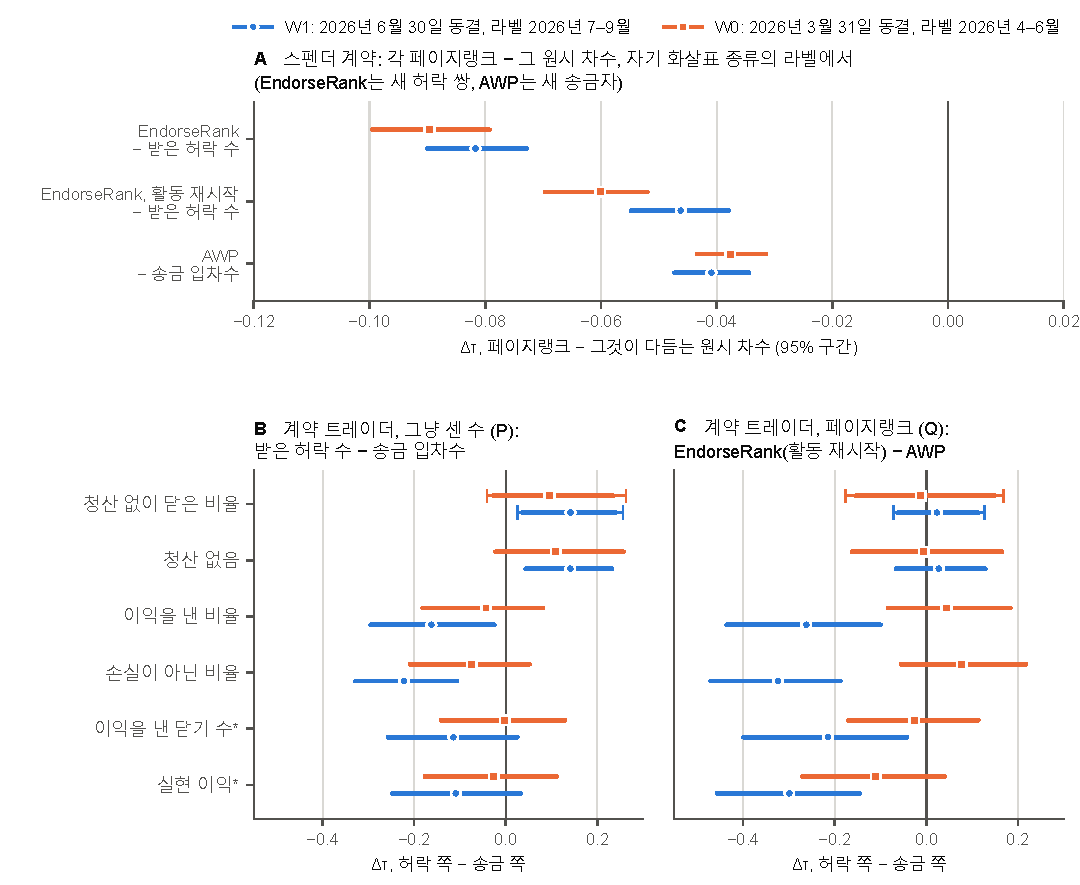
\includegraphics[width=\linewidth]{figures/fig1_ko.pdf}
\caption[페이지랭크 대 원시 차수(스펜더 계약), 허락 쪽 대 송금 쪽(계약 트레이더).]{\textbf{페이지랭크 대 원시 차수(스펜더 계약), 허락 쪽 대 송금 쪽(계약 트레이더).} 점마다 석 달 라벨 기간이 시작할 때 동결한 두 점수의 켄달 $\tau_b$ 짝지은 차이예요. 파란 동그라미는 W1(2026년 6월 30일 동결, 라벨 2026년 7–9월), 주황 네모는 W0(2026년 3월 31일 동결, 라벨 2026년 4–6월)이에요. 굵은 선은 보정하지 않은 95\% 짝지은 부트스트랩 구간이에요. (A) 스펜더 계약(W0 $n=7{,}914$, W1 $7{,}960$; 다시 뽑기 400번): 각 페이지랭크 − 그것이 다듬는 원시 차수. 엔도스랭크 두 변형은 새 허락 쌍에서, AWP는 새 송금자에서 견줬고, 라벨을 안 뒤에 계산했어요. (B) 계약 트레이더(W0 $n=87$, W1 $70$; 다시 뽑기 2,000번): 받은 허락 수 − 송금 입차수(대비 P)를 나중 결과 여섯 개에서. (C) 같은 것을 활동 재시작 엔도스랭크 − AWP(대비 Q)로. (B)와 (C)의 첫 줄에서 끝 눈금이 있는 가는 선은 97.5\% 구간이에요. W1에서는 이것이 등록 규칙의 판정 구간이고, 여기서는 수정 점수에 적용했어요. 별표는 닫기 수에 따라 커지는 두 결과예요. 수정 분석(달러 금액, 다섯 토큰, 동결 직전 12개월의 점수).}
\label{fig1}
\end{figure}

\paragraph{활동 재시작.}
AWP의 활동 재시작을 쓰면, 엔도스랭크는 두 창 모두에서 새 허락 쌍을 균등 재시작 꼴보다 잘 줄 세워요. W0에서 +0.029 [0.023, 0.037], W1에서 +0.035 [0.029, 0.042]만큼이에요. 그래도 여전히 받은 허락 수보다는 낮아요(−0.060 [−0.070, −0.052]와 −0.046 [−0.055, −0.038]). 두 변형은 걷기가 어디서 다시 출발하는지만 달라요. 그러니 이 라벨에서 활동 재시작은 수와의 간격을 좁히지만 메우지는 못해요. 이 비교도 각 창의 라벨을 안 뒤에 했어요.

\paragraph{덮는 범위.}
덮는 범위로는 차수 비교를 설명할 수 없어요. AWP는 동결 전에 송금 화살표가 없던 W0 스펜더 1,342개, 곧 약 6개 가운데 1개에 0점을 줘요. 이 스펜더들은 나중에 새 허락 쌍은 다른 스펜더보다 더 자주 얻었지만(26.7\% 대 20.9\%), 새 송금자는 거의 얻지 못했어요(1.4\% 대 21.3\%). 동결 전에 다른 주소에게서 송금을 받은 스펜더 6,489개로 좁혀도(결과를 안 뒤에 고른 부분 집합), 두 차수 비교의 부호는 그대로예요. AWP − 송금 입차수는 새 송금자에서 −0.051 [−0.059, −0.043], 엔도스랭크 − 받은 허락 수는 새 허락 쌍에서 −0.087 [−0.096, −0.078]이에요.

하지만 덮는 범위가 화살표 종류 사이의 비교는 얼마쯤 설명해요. 그 부분 집합에서 AWP는 새 허락 쌍을 0.328 [0.312, 0.343]으로 줄 세워요. 엔도스랭크(0.299 [0.283, 0.315])보다 위이고 받은 허락 수(0.387 [0.370, 0.402])보다 아래예요. 짝지은 대비는 계산하지 않았어요. 그러니 새 허락 쌍에서 엔도스랭크가 AWP보다 앞선 것은 그 부분 집합 밖의 스펜더에서 와요. AWP가 0점을 준 1,342개가 여기에 들어가요.

\paragraph{동점.}
동점도 양쪽에서 한몫할 수 있어요. 받은 허락 수와 송금 입차수는 동점이 아주 많은 정수예요. 엔도스랭크는 W0 스펜더 7,914개에 서로 다른 점수 7,368개를 주고, 쌍의 0.058\%만 동점이에요. AWP는 그 가운데 1,342개에 똑같이 0점을 주고, 쌍의 2.87\%가 동점이에요. $\tau_b$는 이 둘을 다르게 다루는데, 동점에 흔들리지 않는 비교는 하지 않았어요.

\paragraph{다른 두 라벨.}
계획이 정하지 않은 라벨 두 개를 W0 스펜더에서 더 계산했어요.
\begin{itemize}
\item \textbf{허락 거두기:} 동결 시점에 양수의 허락을 둔 주인 가운데, 라벨 기간에 그 허락을 0으로 바꾼 주인의 수.
\item \textbf{털린 주인:} 새 허락 뒤 몇 시간 안에 같은 토큰이 밖으로 송금된 주인의 수. 휴리스틱으로 세요(S1 Text).
\end{itemize}
모든 점수가 두 라벨을 양의 방향으로 줄 세워요. 허락 거두기는 받은 허락 수를 가장 잘 따르고(0.384 [0.366, 0.399]), 송금 입차수를 가장 못 따라요(0.186 [0.167, 0.209]). 털린 주인의 계수는 송금 입차수의 0.162 [0.143, 0.183]부터 활동 재시작 엔도스랭크의 0.341 [0.325, 0.356]까지예요. 주인들이 더 믿은 계약이라면 허락을 더 자주가 아니라 덜 자주 잃어야 해요. 그러니 이 수들은 보증보다는 주인 활동의 양을 따르고, 어느 것도 증거로 내놓지 않아요.

%----------------------------------------------------------------------
\subsection{깊이 1인 스펜더에서 엔도스랭크가 계산하는 것}
\label{sec:closed}

\begin{yoji}
주인들이 아무에게서도 허락을 받지 않는 스펜더(깊이 1)에서, 엔도스랭크는 정확히 $c\,(1+d\,\delta(v))$, 곧 무게를 다시 단 허락 수예요. 이 식은 깊이 1인 스펜더 모두에서 1\% 안으로 맞고, 더 깊은 스펜더에서는 대부분 벗어나요.
\end{yoji}

한 걸음 추출 때문에 허락 그래프의 점은 대부분 순수한 주인이거나 순수한 스펜더예요. 코호트 계약은 허락을 받기도 하고 다른 계약에 허락을 주기도 하므로 둘 다일 수 있고, 그래서 그래프에는 더 긴 경로도 있어요. 주인들이 허락을 받지 않는 스펜더라면, 엔도스랭크를 식으로 풀어 쓸 수 있어요.

\paragraph{관찰.}
페이지랭크가 감쇠 계수 $d$와 균등 재시작 $\pi_u=1/|V|$로 식~\eqref{eq:pagerank}을 따르고, $r_D$가 매달린 점들의 점수 합이라고 해요. 그러면 들어오는 화살표가 없는 모든 점은 같은 점수를 가져요.
\begin{equation}
\label{eq:c}
c=\frac{1-d+d\,r_D}{|V|}
\end{equation}
그리고 들어오는 이웃 가운데 누구에게도 들어오는 화살표가 없는 점 $v$의 점수는 이래요.
\begin{equation}
\label{eq:closed-form}
r_v=c\,\bigl(1+d\,\delta(v)\bigr),
\qquad
\delta(v)=\sum_{u}\frac{w(u,v)}{o(u)}
\end{equation}
$\delta(v)$는 $v$의 “주인별로 나눈(정규화한) 받은 무게”예요. 주인 $u$마다 자기 허락 무게 가운데 $v$로 가는 몫을 보태요. 그래서 많은 스펜더에게 허락하는 주인은 각 스펜더에 조금씩만 보태요.

\paragraph{끌어내기.}
식~\eqref{eq:pagerank}의 고정점에서 모든 점 $v$는 순간 이동으로 $(1-d)/|V|$를, 매달린 행에서 $d\,r_D/|V|$를 받아요. 둘을 합치면 $c$예요. 여기에 들어오는 이웃에게서 $d\sum_u r_u\,w(u,v)/o(u)$를 더 받아요. 들어오는 화살표가 없는 점은 $c$만 받아요. $v$의 들어오는 이웃 $u$가 모두 그런 점이면, $r_u=c$를 넣어 식~\eqref{eq:closed-form}이 나와요.

이 식은 엄밀한 뜻의 닫힌 식이라기보다 고정점을 한 걸음 펼친 것이에요. $c$가 $r_D$에 달려 있고, $r_D$는 점수 벡터 전체가 정하기 때문이에요. 하지만 $c$는 식이 덮는 모든 스펜더에 공통이므로, 엔도스랭크는 그 스펜더들을 $\delta(v)$와 정확히 같은 순서로 줄 세워요.

이 식은 계산한 점수를 설명해요(표~\ref{tab1}).
\begin{itemize}
\item $\Tobs$의 그래프에서 들어오는 화살표가 없는 모든 점은 부동소수점 오차 안에서 같은 점수 $c=1.93\times10^{-7}$을 가져요.
\item 코호트 스펜더 6,224개 가운데 깊이 1인 5,232개는 모두 식~\eqref{eq:closed-form}과 1\% 안이에요. 나머지 992개는 주인 가운데 허락을 받은 주소가 하나 이상 있는데, 21.9\%만 1\% 안이에요. 모든 스펜더로는 87.5\%예요.
\item $t_1$의 그래프에서는 허락 화살표가 들어오는 W0 스펜더 7,905개 가운데 5,092개가 깊이 1이고, 역시 모두 1\% 안이에요. 이 W0 스펜더 전체로는 70.8\%가 1\% 안이에요.
\item W0 스펜더 코호트에 더 깊은 스펜더가 많은 까닭 하나는, W0 코호트 밖의 계약도 들어가기 때문이에요. 그런 계약은 코호트 계약이 준 허락으로만 자료에 들어와요.
\end{itemize}

이로부터 두 가지가 나와요.
\begin{enumerate}
\item \textbf{깊이 1인 스펜더에서 걷기는 허락한 주인들의 무게를 다시 다는 일만 해요.} 허락은 최근이고 클수록(무게 1까지) 무겁고, 그 주인이 허락을 많은 스펜더에 나눠 줄수록 가벼워요. 이 무게와 나눗셈을 빼면, 그런 스펜더에 대해 엔도스랭크와 수는 같은 정보를 담고, 퍼뜨림이 더 보탤 것이 없어요. 어느 무게 때문에 엔도스랭크가 나중 허락과의 일치를 잃었는지는 따로 떼어 보지 않았어요.
\item \textbf{더 긴 경로가 있어요.} $\Tobs$의 코호트 스펜더 약 6개 가운데 1개, W0 스펜더 약 3개 가운데 1개는, 다른 주소에게서 허락을 받는 주인에게서 허락을 받아요. 그리고 그런 스펜더의 점수는 대부분 닫힌 식과 1\% 넘게 달라요. 그러니 이 그래프에서도 여러 단계에 걸친 퍼뜨림은 일어나요. 하지만 그 퍼뜨림이 기간 밖에서 엔도스랭크를 원시 차수보다 낫게 만들지는 못했어요. 균등 재시작으로도, 활동 재시작으로도요. 순환이 있는 송금 그래프를 걷는 AWP에는 이에 맞먹는 닫힌 식이 없어요.
\end{enumerate}

\begin{puri}[$\delta(v)$를 작은 예로 보면]
주인이 스펜더 \ill{4}곳에 똑같은 무게로 허락했다면, 그 주인은 스펜더마다 $\delta$에 \ill{1/4}씩 보태요. 스펜더 한 곳에만 허락한 주인은 그 스펜더에 1을 통째로 보태요. 그래서 허락한 주인 수가 같아도, 한 곳에만 허락하는 주인이 많은 스펜더가 더 높은 점수를 받아요. 같은 주인의 허락끼리는, 최근이고 금액이 큰 허락이 더 큰 몫을 가져가요. 깊이 1인 스펜더에서 엔도스랭크의 순서는 이 $\delta(v)$의 순서와 똑같아요.
\end{puri}

%----------------------------------------------------------------------
\subsection{어느 화살표로도 만들지 않은 결과}
\label{sec:neutral}

\begin{yoji}
GMX V2 계약 트레이더의 나중 청산 피하기에서, W1의 P는 +0.141(97.5\% 구간 [0.026, 0.256])로 R1의 세 조건을 모두 만족했어요. 재분석의 판정이고, 등록 분석에서는 R1이 성립하지 않았어요. Q는 판가름 나지 않아 R2는 성립하지 않고, 거래 성적을 나타내는 비율에서는 송금 쪽이 앞서 R3이 적용돼요. 허락을 받은 트레이더는 한 번도 청산되지 않았어요.
\end{yoji}

이 소절의 모든 결과는 등록한 쌍, 규칙, 문구를 등록 분석의 결과를 안 뒤에 수정 점수에 적용한 것이고, 재분석이에요. 표~\ref{tab4}는 청산 없이 닫은 비율에서의 대비를, 그림~\ref{fig1}B와 C는 라벨 여섯 개 모두를 보여 줘요. 계약 트레이더가 W1에 70개, W0에 87개뿐이라 여기의 구간은 모두 넓어요. W1의 트레이더 70개 가운데 9개는 청산을 한 번 이상 겪었고, 1개는 모든 닫기가 청산이었어요.

\begin{table}[!htbp]
\centering
\caption{계약 트레이더의 나중 청산 없이 닫은 비율에서, 허락 쪽 점수 − 송금 쪽 점수.}
\label{tab4}
\footnotesize
\setlength{\tabcolsep}{4pt}
\begin{tabular}{@{}lccccc@{}}
\toprule
대비($a-b$) & $\tau(a)$ & $\tau(b)$ & $\dt$ & 95\% 구간 & 97.5\% 구간 \\
\midrule
\multicolumn{6}{@{}l}{\emph{W1: 2026년 6월 30일 동결, 라벨 2026년 7–9월(계약 트레이더 $n=70$)}} \\
P: 받은 허락 수 − 송금 입차수 & 0.394 & 0.253 & +0.141 & [0.037, 0.240] & [0.026, 0.256] \\
\quad P, 닫은 횟수로 층화 & 0.381 & 0.236 & +0.145 & [0.040, 0.328] & – \\
Q: EndorseRank(활동 재시작) − AWP & 0.286 & 0.263 & +0.023 & [−0.062, 0.113] & [−0.071, 0.127] \\
\quad Q, 닫은 횟수로 층화 & 0.273 & 0.238 & +0.034 & [−0.096, 0.171] & – \\
EndorseRank − AWP & 0.297 & 0.263 & +0.034 & [−0.067, 0.134] & – \\
EndorseRank − 받은 허락 수$^{a}$ & 0.297 & 0.394 & −0.097 & [−0.174, −0.009] & – \\
C-PR($\lambda{=}1$) − C-PR($\lambda{=}0$)$^{b}$ & 0.302 & 0.282 & +0.019 & [−0.093, 0.128] & – \\
C-PR($\lambda{=}0$) − AWP$^{b}$ & 0.282 & 0.263 & +0.019 & [−0.031, 0.066] & – \\
\midrule
\multicolumn{6}{@{}l}{\emph{W0: 2026년 3월 31일 동결, 라벨 2026년 4–6월(계약 트레이더 $n=87$)}} \\
P: 받은 허락 수 − 송금 입차수 & 0.345 & 0.249 & +0.095 & [−0.027, 0.234] & [−0.041, 0.263] \\
\quad P, 닫은 횟수로 층화 & 0.342 & 0.253 & +0.089 & [−0.025, 0.252] & – \\
Q: EndorseRank(활동 재시작) − AWP & 0.242 & 0.254 & −0.012 & [−0.153, 0.149] & [−0.177, 0.168] \\
\quad Q, 닫은 횟수로 층화 & 0.229 & 0.265 & −0.036 & [−0.186, 0.145] & – \\
EndorseRank − AWP & 0.236 & 0.254 & −0.019 & [−0.173, 0.144] & – \\
EndorseRank − 받은 허락 수$^{a}$ & 0.236 & 0.345 & −0.109 & [−0.196, −0.018] & – \\
C-PR($\lambda{=}1$) − C-PR($\lambda{=}0$)$^{b}$ & 0.237 & 0.294 & −0.057 & [−0.209, 0.092] & – \\
C-PR($\lambda{=}0$) − AWP$^{b}$ & 0.294 & 0.254 & +0.040 & [−0.023, 0.098] & – \\
\bottomrule
\end{tabular}

\begin{minipage}{\linewidth}\footnotesize\raggedright\vspace{0.4em}
라벨 기간에 GMX~V2에서 셋 이상 닫은 계약 트레이더에서, 점수 $a$와 $b$의 켄달 $\tau_b$와 그 차이예요. 짝지은 계약 부트스트랩 2,000번(시드 42). 쌍들, 본페로니 97.5\% 구간을 쓰는 P와 Q, 층화한 행, 규칙 R1–R3은 이 연구가 W1의 로그를 추출하기 전에 W1에 대해 등록했어요. 여기서는 등록 분석의 결과를 안 뒤에 수정 점수에 적용했으므로, 어느 행도 등록한 시험이 아니에요. 규칙에 들어가는 것은 W1의 P와 Q의 97.5\% 구간뿐이고, 다른 구간은 모두 보정하지 않았어요. 층화한 행은 라벨 기간 닫기 수 3–4, 5–9, 10–24, 25 이상의 층 안에서 구한 $\tau_b$를 계약 쌍의 수로 무게를 달아 합친 값이에요. $^{a}$등록 문서에는 이름이 없고, 등록과 함께 커밋한 코드가 계산했어요. $^{b}$금액 무게를 단 허락 층과 송금 층을 각각 혼자, 고르게 다시 출발하며 걸은 점수예요. 출처: \texttt{analysis/neutral-label/results.json}, \texttt{analyses.revised.windows}. 라벨 여섯 개 모두는 보조 자료 S2 Table에 있어요.
\end{minipage}
\end{table}

\paragraph{수(R1 성립).}
W1 트레이더에서 받은 허락 수의 최댓값은 1이에요. 그래서 P는 사실상 동결 시점에 허락을 받아 둔 트레이더 37개와 그렇지 않은 33개를 견줘요. 받은 허락 수는 나중의 청산 없이 닫은 비율을 $\tau=0.394$ [0.265, 0.518]로, 송금 입차수는 0.253 [0.117, 0.379]로 줄 세워요. 송금 수도 이 결과를 얼마쯤 줄 세우는 거예요.
\begin{itemize}
\item P는 +0.141 [0.037, 0.240]이고, 97.5\% 구간 [0.026, 0.256]이 0보다 위에 있어요.
\item 닫은 횟수로 층화한 P는 +0.145 [0.040, 0.328]이에요.
\item W0에서 P=+0.095(97.5\% 구간 [−0.041, 0.263])로, R1이 요구하는 대로 양수예요. 다만 판가름 나지는 않았어요.
\end{itemize}
R1의 세 조건이 모두 맞으므로, 이 경우의 등록 문구가 적용돼요: \emph{동결 시점의 허락 수가 나중의 청산 피하기에서 계약 트레이더를 송금 수보다 더 잘 줄 세웠다.} 점수(달러 금액, 다섯 토큰, 동결 직전 12개월의 점수 기간)는 등록 분석의 결과를 안 뒤에 정의했어요. 그래서 이 판정은 재분석이지 등록한 시험의 결과가 아니에요. 등록 분석에서는 R1이 성립하지 않았어요(표~\ref{tab6}).

\paragraph{페이지랭크(R2 성립 안 함).}
Q(활동 재시작 엔도스랭크 − AWP)는 W1에서 +0.023(97.5\% 구간 [−0.071, 0.127]), W0에서 −0.012(97.5\% 구간 [−0.177, 0.168])예요. 등록 문구로는, \emph{페이지랭크 버전은 판가름 나지 않았다.} W1의 Q의 97.5\% 구간은 폭이 0.20이에요. 그러니 이 표본 크기에서는 0.1 이하의 추정값, 곧 스펜더 라벨에서 본 모든 차수 대비만 한 크기(표~\ref{tab3})는 판가름 나지 않았을 거예요.

다른 쌍도 판가름 나지 않았어요. 엔도스랭크 − AWP는 W1에서 +0.034 [−0.067, 0.134], W0에서 −0.019 [−0.173, 0.144]이고, 금액 무게 층끼리는 +0.019 [−0.093, 0.128]과 −0.057 [−0.209, 0.092] 차이 나요. 등록 문서가 이름 붙이지 않은 대비에서, 엔도스랭크는 두 창 모두 허락 수보다 낮아요. W1에서 −0.097 [−0.174, −0.009], W0에서 −0.109 [−0.196, −0.018]이에요. 스펜더 라벨에서처럼 여기서도 균등 재시작 걷기는 자기가 다듬는 수에 져요.

\paragraph{다른 라벨(R3 적용).}
거래량에 따라 커지지 않는 두 비율은 반대로 가요. W1에서는 두 비율 모두에서 송금 수가 허락 수보다 트레이더를 더 잘 줄 세워요. P는 이익을 낸 비율에서 $\dt=-0.162$ [−0.295, −0.025], 손실이 아닌 비율에서 −0.222 [−0.328, −0.106]이에요. 그래서 R3이 적용되고, 등록 문구는 이래요: \emph{신호는 강제 청산을 피하는 일에 관한 것이지, 거래의 성공에 관한 것이 아니다.} 청산된 닫기는 손실이 아닌 것으로 세므로, 손실이 아닌 비율에서 생긴 간격의 일부는 정의에서 저절로 나와요. 이익을 낸 비율은 그런 닫기를 이익이 아닌 것으로 세므로, R3은 주로 이 비율에 기대요.

나머지 라벨은 이래요.
\begin{itemize}
\item 청산 없음 표시에서 P는 W1에서 +0.141 [0.044, 0.232], W0에서 +0.109 [−0.022, 0.257]이에요.
\item 거래량에 따라 커지는 두 결과에서는, W1의 페이지랭크 쌍이 송금 쪽을 편들어요. Q는 이익을 낸 닫기 수에서 −0.215 [−0.399, −0.042], 실현 이익에서 −0.299 [−0.457, −0.146]이고, 실현 이익에서 AWP는 0.280 [0.111, 0.435]에 이르러요. W1에서는 같은 쌍들이 두 비율에서도 송금 쪽을 편들어요(S2 Table).
\item W0에서는 허락 대 송금의 어느 쌍도 두 비율에서 판가름 나지 않았어요. 거래 성공을 나타내는 라벨 넷 가운데서는, 실현 이익에서 금액 무게 층끼리의 쌍만 판가름 났어요(−0.257 [−0.447, −0.071]).
\item 등록 문서가 이름 붙이지 않은 대비인 엔도스랭크 − 받은 허락 수는 W0의 이익을 낸 비율에서 +0.113 [0.022, 0.210], W0의 손실이 아닌 비율에서 +0.121 [0.034, 0.211]이에요.
\end{itemize}

\paragraph{허락을 받은 트레이더는 누구인가요?}
허락을 받은 트레이더는 두 창 모두에서 하나도 청산되지 않았어요(W1 37개 가운데 37개, W0 39개 가운데 39개). 다른 트레이더는 72.7\%와 75.0\%가 청산 없이 지냈어요(표~\ref{tab5}). 허락을 받은 트레이더가 그저 덜 활발했던 것도 아니에요. 그들은 포지션을 더 많이 닫았고(중앙값 W1 24 대 11, W0 30 대 10), 이익을 낸 비율과 손실이 아닌 비율의 평균은 더 낮았어요(W1에서 0.325 대 0.479, 0.433 대 0.644). R3 뒤에 있는 모양이에요.

허락한 주인 수가 가장 많은 허락을 받은 트레이더 10개를 빼도, P는 W1에서 +0.155 [0.032, 0.276], W0에서 +0.088 [−0.048, 0.240]이에요. 차수가 거의 다 1로 같아서, 빼는 10개는 점 순서로 골랐어요. 두 창의 모든 트레이더가 계약이므로, 허락을 받은 쪽과 다른 쪽으로 나눈 것은 계정 종류로 나눈 것이 아니에요.

표~\ref{tab5}의 모든 줄에 들어맞을 설명이 하나 있어요. 허락을 받은 트레이더는, 남들이 자기 토큰을 옮기도록 허락하는 금고(vault)나 위탁 운용 계약이면서, 낮은 레버리지로 거래하고 포지션을 자주 조정하는 계약일 수 있어요. 그렇다면 청산은 드물고, 일부 닫기가 많고, 이익을 낸 비율은 수수할 거예요. 자료에는 레버리지도 각 계약의 구실도 없으므로, 이 설명은 시험하지 않았어요.

\begin{table}[!htbp]
\centering
\caption{동결 시점에 허락을 받은 계약 트레이더(허락을 받은 트레이더)와 다른 모든 트레이더.}
\label{tab5}
\small
\begin{tabular}{@{}L{5.6cm}cccc@{}}
\toprule
 & \multicolumn{2}{c}{W1(2026년 7–9월)} & \multicolumn{2}{c}{W0(2026년 4–6월)} \\
\cmidrule(lr){2-3}\cmidrule(lr){4-5}
 & 허락 받음 & 다른 트레이더 & 허락 받음 & 다른 트레이더 \\
\midrule
트레이더 수 & 37 & 33 & 39 & 48 \\
청산이 하나도 없었던 몫 & 1.000 & 0.727 & 1.000 & 0.750 \\
청산 없이 닫은 비율의 평균 & 1.000 & 0.878 & 1.000 & 0.919 \\
이익을 낸 비율의 평균 & 0.325 & 0.479 & 0.359 & 0.474 \\
손실이 아닌 비율의 평균 & 0.433 & 0.644 & 0.401 & 0.607 \\
라벨 기간 닫기 수의 중앙값 & 24.0 & 11.0 & 30.0 & 10.0 \\
동결 시점 받은 허락 수의 최댓값 & 1 & 0 & 3 & 0 \\
\midrule
받은 허락 수가 가장 큰 허락 받은 트레이더 10개를 뺀 P & \multicolumn{2}{c}{+0.155 [0.032, 0.276]($n=60$)} & \multicolumn{2}{c}{+0.088 [−0.048, 0.240]($n=77$)} \\
\bottomrule
\end{tabular}

\begin{minipage}{\linewidth}\footnotesize\raggedright\vspace{0.4em}
허락을 받은 트레이더는 동결 시점의 받은 허락 수가 0보다 커요. 두 창의 모든 트레이더는 계약 코드를 가져요. 이 비교와 영향 점검(청산 없이 닫은 비율의 P, 짝지은 다시 뽑기 2,000번의 95\% 구간)은 표~\ref{tab4}의 대비와 함께 등록했고, 여기서는 수정 점수에 적용했어요. 받은 허락 수가 같으면, 빼는 10개는 점 순서로 골라요. 출처: \texttt{analysis/neutral-label/results.json}의 \texttt{recipients}, \texttt{influence\_without\_top10}.
\end{minipage}
\end{table}

%----------------------------------------------------------------------
\subsection{등록 분석}
\label{sec:registered}

\begin{yoji}
원래 단위, 모든 ERC-20 토큰, 2023년 10월 1일부터의 모든 사건으로 점수를 만든 등록 분석은 R2와 R3에서 같은 판정을 냈지만, R1은 성립하지 않았어요. 이 연구가 판정 자료를 추출하기 전에 정한 시험의 결과는 등록 분석의 판정뿐이에요.
\end{yoji}

등록 분석은 원래 단위, 모든 ERC-20 토큰, 2023년 10월 1일부터의 모든 사건으로 만든 점수, 그리고 계획의 코호트(계약 27,844개)를 썼어요. 이 분석은 R2와 R3에서는 같은 판정에, R1에서는 다른 판정에 이르렀어요(표~\ref{tab6}).
\begin{itemize}
\item W1의 P는 +0.063 [−0.026, 0.148], 97.5\% 구간은 [−0.040, 0.158]이었고, 층화한 구간도 0을 포함했어요.
\item W1의 Q는 +0.051, 97.5\% 구간은 [−0.104, 0.232]였어요.
\item R1과 R2는 성립하지 않았고, R3은 적용됐어요. 이것이 등록 분석의 결과예요.
\end{itemize}
그러니 수정 분석에서 그냥 센 수의 수준에서 앞선 것이, 두 분석이 갈리는 단 하나의 판정이에요. 그리고 이 연구가 판정할 자료를 추출하기 전에 정한 시험의 결과는 등록 분석의 판정뿐이에요.

두 분석은 어느 규칙도 판정하지 않는 차수 대비 두 곳에서도 달라요. 등록 분석에서 AWP는 두 창 모두 송금 입차수보다 위였어요(+0.038 [0.035, 0.042]와 +0.020 [0.016, 0.023]). 활동 변형도 받은 허락 수보다 위였고, 각 구간이 0을 포함하지 않았어요. 수정 분석에서는 둘 다 자기 수보다 아래예요. 엔도스랭크는 두 분석 모두에서 받은 허락 수보다 낮았고, 두 분석 모두에서 깊이 1인 스펜더가 모두 닫힌 식에 맞았어요. 청산 없이 닫은 비율에서 허락 대 송금의 페이지랭크 쌍(Q, 엔도스랭크 − AWP, 금액 무게 층)은 등록 분석의 두 창 모두에서 양수였어요. 수정 분석에서는 W1에서 양수, W0에서 음수이고, 모두 구간이 0을 포함해요(표~\ref{tab6}).

\begin{table}[!htbp]
\centering
\caption{등록 분석과 수정 분석을 나란히.}
\label{tab6}
\footnotesize
\begin{tabular}{@{}L{6.4cm}cc@{}}
\toprule
 & 등록 분석 & 수정 분석(재분석) \\
\midrule
\multicolumn{3}{@{}l}{\emph{자료와 같은 기간}} \\
금액; 토큰 & 원래 단위; 모든 ERC-20 & 달러; 다섯 토큰 \\
$\Tobs$의 점수에 쓴 사건 & \begin{tabular}[t]{@{}c@{}}2023년 10월 1일 –\\ 2026년 6월 30일\end{tabular} & \begin{tabular}[t]{@{}c@{}}2025년 7월 1일 –\\ 2026년 6월 30일\end{tabular} \\
$t_1$의 점수에 쓴 사건 & \begin{tabular}[t]{@{}c@{}}2023년 10월 1일 –\\ 2026년 3월 31일\end{tabular} & \begin{tabular}[t]{@{}c@{}}2025년 4월 1일 –\\ 2026년 3월 31일\end{tabular} \\
매칭 코호트(계약) & 27,844 & 6,483 \\
$\Tobs$의 허락 / 송금 화살표 & 22,321,470 / 59,737,617 & 3,808,949 / 8,426,124 \\
EndorseRank, 허락 가족 & 0.481 [0.476, 0.487] & 0.560 [0.548, 0.571] \\
AWP, 송금 가족 & 0.447 [0.440, 0.453] & 0.736 [0.728, 0.744] \\
EndorseRank와 AWP 사이의 $\tau_b$ & 0.217 [0.209, 0.225] & 0.199 [0.181, 0.221] \\
식~\eqref{eq:closed-form}과 1\% 안: 깊이 1 / 모든 스펜더 & 100.0\% / 86.4\% & 100.0\% / 87.5\% \\
\midrule
\multicolumn{3}{@{}l}{\emph{스펜더 홀드아웃, 페이지랭크 − 그 원시 차수(라벨을 안 뒤에 계산)}} \\
스펜더 코호트, W0 / W1 & 33,101 / 34,587 & 7,914 / 7,960 \\
W0: EndorseRank − 받은 허락 수, 새 허락 쌍 & −0.011 [−0.016, −0.006] & −0.090 [−0.100, −0.079] \\
W0: EndorseRank(활동) − 받은 허락 수 & +0.043 [0.036, 0.049] & −0.060 [−0.070, −0.052] \\
W0: AWP − 송금 입차수, 새 송금자 & +0.038 [0.035, 0.042] & −0.038 [−0.043, −0.032] \\
W1: EndorseRank − 받은 허락 수, 새 허락 쌍 & −0.029 [−0.032, −0.025] & −0.082 [−0.090, −0.073] \\
W1: EndorseRank(활동) − 받은 허락 수 & +0.018 [0.012, 0.023] & −0.046 [−0.055, −0.038] \\
W1: AWP − 송금 입차수, 새 송금자 & +0.020 [0.016, 0.023] & −0.041 [−0.047, −0.034] \\
\midrule
\multicolumn{3}{@{}l}{\emph{계약 트레이더, 청산 없이 닫은 비율(등록한 쌍과 규칙)}} \\
트레이더 코호트, W1 / W0 & 70 / 88 & 70 / 87 \\
P, W1, 95\% 구간 & +0.063 [−0.026, 0.148] & +0.141 [0.037, 0.240] \\
P, W1, 97.5\% 구간 & +0.063 [−0.040, 0.158] & +0.141 [0.026, 0.256] \\
층화한 P, W1, 95\% 구간 & +0.113 [−0.021, 0.238] & +0.145 [0.040, 0.328] \\
P, W0 & +0.252 [0.093, 0.413] & +0.095 [−0.027, 0.234] \\
Q, W1, 97.5\% 구간 & +0.051 [−0.104, 0.232] & +0.023 [−0.071, 0.127] \\
Q, W0 & +0.062 [−0.078, 0.219] & −0.012 [−0.153, 0.149] \\
EndorseRank − AWP, W1 & +0.066 [−0.069, 0.227] & +0.034 [−0.067, 0.134] \\
EndorseRank − AWP, W0 & +0.062 [−0.079, 0.217] & −0.019 [−0.173, 0.144] \\
C-PR($\lambda{=}1$) − C-PR($\lambda{=}0$), W1 & +0.171 [−0.083, 0.438] & +0.019 [−0.093, 0.128] \\
C-PR($\lambda{=}1$) − C-PR($\lambda{=}0$), W0 & +0.205 [−0.041, 0.437] & −0.057 [−0.209, 0.092] \\
R1(그냥 센 수의 수준에서 앞섬) & 성립 안 함 & 성립 \\
R2(페이지랭크 수준의 앞섬) & 성립 안 함 & 성립 안 함 \\
R3(청산 피하기에만 해당) & 적용 & 적용 \\
\bottomrule
\end{tabular}

\begin{minipage}{\linewidth}\footnotesize\raggedright\vspace{0.4em}
등록 분석은 커밋한 분석 계획과 W1 등록을 그대로 따르고, 2023년 10월 1일부터의 모든 사건으로 점수를 만들어요. 그 값과 판정이 등록된 결과인 곳은 등록 문서의 규칙이 판정하는 곳(P, Q, R1–R3)뿐이고, 다른 트레이더 행은 규칙을 판정하지 않는 등록 쌍이에요. 수정 분석은 금액을 다섯 토큰의 달러 값으로 매기고, 모든 점수를 동결 직전 12개월의 사건으로 만들어요. 이 정의는 등록된 결과를 모두 안 뒤에 정했으므로, 수정 분석의 판정은 나중에 정의한 점수에 등록 규칙을 적용한 것이고 등록한 시험이 아니에요. 차수 대비는 두 분석 모두에서 어느 규칙도 판정하지 않아요. 97.5\%라고 적지 않은 값은 $\dt$와 95\% 구간이에요(짝지은 다시 뽑기 스펜더 400번, 트레이더 2,000번, 시드 42). 출처: 각 분석의 같은 기간, \texttt{holdout-w0}, \texttt{registered-w1}, \texttt{window-w1} 요약과 \texttt{supplementary.json}(\texttt{phd\_works}), \texttt{analysis/closed-form/closed\_form\_check.json}, \texttt{analysis/neutral-label/results.json}.
\end{minipage}
\end{table}

%----------------------------------------------------------------------
\subsection{계산 비용}

\begin{yoji}
같은 풀이 프로그램으로 AWP는 엔도스랭크보다 3.21배 오래 걸렸어요(화살표 수는 2.21배). 시간 차이는 송금 그래프의 크기와 반복 횟수에서 와요.
\end{yoji}

같은 풀이 프로그램과 같은 설정으로 시간을 잰 실행 다섯 번의 평균은 이래요.
\begin{itemize}
\item 엔도스랭크의 풀이 그래프(점 2,513,982개, 화살표 3,808,949개): 2.66초, 표준편차 0.11초.
\item AWP의 풀이 그래프(점 3,601,727개, 화살표 8,426,124개): 8.53초, 표준편차 0.62초.
\end{itemize}
AWP는 화살표 비 2.21에서 3.21배 오래 걸렸어요. 반복도 더 많이 필요했고(94번 대 57번), 최대 메모리는 663.7~MB 대 325.3~MB였어요. 행렬 조립과 거듭제곱 반복 한 번은 화살표 수에 비례해요~\cite{leskovec2020mining}. 그러니 시간 차이는 송금 그래프의 크기와 그 그래프에서 걷기에 필요한 반복 수에서 오고(벤치마크는 둘을 나누지 않았어요), 알고리즘의 어떤 성질에서 오지 않아요. 송금 화살표도 쓰는 걷기는 모두 그 값을 치러요. 짝 원고의 섞은 걷기는 두 화살표 집합을 함께 쓰는데(화살표 10,562,390개) 11.56초 걸렸어요.

%======================================================================
\section{논의}

%----------------------------------------------------------------------
\subsection{화살표 종류가 어떤 나중 손님을 줄 세울지 정해요. 어느 걷기도 원시 차수를 넘지 못했어요}

\begin{yoji}
어떤 화살표를 고르느냐는 계약 평판 점수가 무엇을 따라가게 할지를 고르는 일이에요. 고른 화살표를 따라 퍼뜨려도 원시 차수보다 나아지지 않았어요(라벨을 안 뒤에 한 비교예요). 대부분의 스펜더에서 엔도스랭크는 무게를 다시 단 허락 수예요.
\end{yoji}

두 화살표 종류는 서로 다른 것을 재고, 기간 밖 결과가 두 창 모두에서 이것을 보여 줘요. 허락으로 만든 점수는 어느 계약이 나중에 새 허락을 얻을지를, 송금으로 만든 점수는 어느 계약이 나중에 새 송금자를 얻을지를 줄 세워요. 그러니 화살표를 고르는 것은, 계약의 평판 점수가 무엇을 따라가야 하는지를 정하는 일이에요.

고른 화살표를 따라 점수를 퍼뜨려도 어느 쪽에서도 보탠 것이 없었어요. 라벨을 안 뒤에 한 비교에서, AWP는 두 창 모두 송금 수보다, 엔도스랭크는 두 창 모두 허락 수보다 낮았어요. 송금을 받은 적 있는 스펜더로 좁힌 집합에서도 W0에서 같았어요. 수를 이기기 어렵다는 것은 선호적 연결(이미 많이 이어진 점에 새 화살표가 더 붙는 현상)과 링크 예측의 관행을 생각하면 놀랍지 않아요~\cite{barabasi1999scaling,libennowell2007link}. 그런데도 온체인 평판 연구는 이것을 거의 시험하지 않아요. 걷기를 다른 걷기와, 또는 자기 화살표로 만든 통계와만 견줘요~\cite{do2023awp}.

닫힌 식은 대부분의 스펜더에서 엔도스랭크가 무엇을 계산하는지 알려 줘요. 허락 수인데, 허락마다 얼마나 최근이고 얼마나 큰지로 크기를 정한 뒤, 그 주인의 허락 무게 합으로 나눈 것이에요. 이 정규화는 주인들이 다른 계약에도 많이 허락하는 스펜더를 낮춰요. 이 정규화 때문인지, 아니면 시간 무게나 금액 무게 때문인지, 무엇이 엔도스랭크와 나중 허락의 일치를 떨어뜨렸는지는 따로 떼어 보지 않았어요.

활동 재시작 변형은 다시 출발 몫을 허락을 가장 많이 주는 주인에게 보내요. 이 변형은 두 창 모두에서 나중의 허락 쌍을 엔도스랭크보다 잘 줄 세웠지만, 여전히 수보다는 아래였어요(표~\ref{tab3}). 그러니 이 비교들에서(모두 라벨을 안 뒤에 한 비교예요) 활발한 주인에서의 다시 출발은 수와의 간격을 좁혔지만 메우지 못했어요. AWP는 논문에 발표된 다시 출발 규칙으로만 돌렸고, 역시 모자랐어요.

걷기가 무게를 다시 단 수보다 더 무언가인 곳에서 퍼뜨림이 수에 무엇을 보태는지 알려면, 두 걸음 이상 바깥까지 추출한 표본과, 아직 추출하지 않은 창에서의 등록한 시험이 필요해요. 그때는 걷기가 무게 단 수로 줄어드는 깊이 1인 스펜더와, 퍼뜨림이 중요할 수 있는 더 깊은 스펜더를 나눠 보고해야 해요.

%----------------------------------------------------------------------
\subsection{트레이더 비교가 보여 주는 것}

\begin{yoji}
재분석에서 허락 수는 주 결과(청산 피하기)에서 송금 수와 갈렸어요. 하지만 이 앞섬은 등록한 시험의 결과가 아니고, 허락을 받은 트레이더 37개와 다른 33개에 기대요. 허락이 신용이나 거래 실력을 잰다는 근거는 없어요.
\end{yoji}

트레이더 결과는 거래소가 기록하고, 어느 그래프도 기록하지 않아요. 이 자료에서 어느 그래프로도 만들지 않은 결과는 이것뿐이에요. 다만 동결 전의 GMX 지급은 송금 그래프에 나타날 수 있어요.

주 결과에서, 이 재분석의 허락 수는 송금 수와 갈렸어요.
\begin{itemize}
\item W1에서 허락 수는 나중의 청산 피하기를 $\tau=0.394$ [0.265, 0.518]로, 송금 수는 0.253 [0.117, 0.379]로 줄 세웠어요. 둘의 차이 P는 97.5\% 구간이 0보다 위였고, 닫은 횟수로 층화한 P도 95\% 구간이 0보다 위였어요.
\item 보조 창 W0은 라벨 기간이 W1의 점수 기간 안에 들어 있어요. 여기서 P는 양수였지만 97.5\% 구간이 0 아래까지 내려왔어요. R1은 W0에서 양수인 추정값만 요구했어요.
\end{itemize}
이 결과에는 두 가지 테두리가 있어요.
\begin{itemize}
\item 점수(달러 금액, 다섯 토큰, 동결 직전 12개월의 점수 기간)는 등록 분석의 결과를 안 뒤에 정의했고, 등록 분석에서는 W1의 P의 97.5\% 구간이 0 아래까지 내려왔어요. 그러니 이 앞섬은 재분석의 발견이지 등록한 시험의 발견이 아니에요.
\item 이 앞섬은 허락을 받은 트레이더 37개와 다른 트레이더 33개에 기대고, 이들은 모두 계약이에요.
\end{itemize}
페이지랭크 쌍은 어느 분석의 어느 창에서도 판가름 나지 않았어요(표~\ref{tab6}). 거래 성공을 나타내는 결과에서는, 허락 쪽 점수와 송금 쪽 점수의 차이가 판가름 난 곳마다 송금 쪽이 앞섰어요. 그리고 어느 점수도 두 창 가운데 어디서도 이익을 낸 비율을 0보다 위의 구간으로 줄 세우지 못했어요.

규칙을 넘어서 보이는 모양은 묘사일 뿐이에요. 허락을 받은 계약은 두 창 모두에서 하나도 청산되지 않았어요. 이 모양은 수십 개의 계약에 기대고, 누가 허락했는지보다 그 계약이 무엇인지를 반영할 수 있어요. 또한 거래 장소가 동결 전에 이미 아는 것, 예를 들어 계약 자신의 청산 기록, 닫은 횟수, 레버리지와 견주지 않았어요. 그러니 과거 행동을 넘어서는 값을 보여 주지 않아요. 그리고 여기의 어떤 결과도 허락이 신용도, 부도 위험, 거래 실력을 잰다고 말해 주지 않아요. 증거금 거래소나 대출 서비스가 허락 수로 계약 상대를 거를 수 있을지는 열린 질문이에요. 그러려면 아직 추출하지 않은 창에서, 더 많은 계약 트레이더로, 과거 행동을 통제한 등록한 시험이 필요해요.

%----------------------------------------------------------------------
\subsection{온체인 평판을 평가하는 방법에 주는 시사점}

\begin{yoji}
걷기 옆에는 늘 원시 차수를 보고하고, 점수는 라벨보다 먼저 동결하고, 어느 화살표로도 만들지 않은 결과로 견주고, 비교마다 언제 정했는지 밝히라는 네 가지 권고예요.
\end{yoji}

이 연구는 온체인 평판 점수를 평가할 때의 네 가지 관행을 권해요.
\begin{enumerate}
\item \textbf{걷기마다 그 옆에 원시 차수를 보고해요.} 여기서 어느 걷기도 기간 밖에서 자기 원시 차수를 이기지 못했어요. 자기 화살표로 만든 통계와만 견준 걷기~\cite{do2023awp}로는 이것을 보일 수 없었을 거예요.
\item \textbf{어떤 라벨을 세기 전에 점수를 동결해요.}
\item \textbf{어느 쪽으로도 만들지 않은 결과에서 화살표 종류를 견줘요.} 각 화살표 종류는 설계상 자기 구성개념의 라벨에서 앞서기 때문이에요~\cite{cronbach1955construct}. 그리고 그 결과가 그래프와 얼마나 떨어져 있는지도 확인해요.
\item \textbf{비교마다 자료를 기준으로 언제 정했는지 밝히고, 결과를 안 뒤에 정의한 분석은 등록한 분석 옆에 둬요}~\cite{nosek2018preregistration}. 여기서 두 분석은 R2와 R3에서 같았어요. 하지만 청산 피하기에서 그냥 센 수의 수준에서 앞선 것은 나중에 정의한 분석(달러 금액, 다섯 토큰, 동결 직전 12개월의 점수 기간)에서만 성립하고, AWP와 활동 변형이 자기 수보다 앞선 것은 등록 분석에서만 나타나요.
\end{enumerate}

%----------------------------------------------------------------------
\subsection{실제 쓰임}

\begin{yoji}
지갑은 주인에게 “이 계약에 양수의 허락을 둔 서로 다른 주인 수”를 보여 줄 수 있어요. 하지만 그 수는 얼마나 널리 허락받았는지를 알려 줄 뿐, 안전하다는 뜻이 아니에요. 그리고 값싸게 부풀릴 수 있어요.
\end{yoji}

어떤 계약에 허락할지 정하는 주인에게, 이미 그 계약에 양수의 허락을 둔 서로 다른 주인 수를 보여 줄 수 있어요. 지갑 프로그램이 계산할 수 있는 공개된 수예요. 기간 밖에서 엔도스랭크는, 균등 재시작이든 활동 재시작이든, 나중의 새 허락 쌍을 이 수만큼 잘 줄 세우지 못했어요.

이런 수는 계약이 이미 얼마나 널리 허락받았는지를 주인에게 알려 줄 뿐, 그 계약이 허락으로 무엇을 할지는 알려 주지 않아요.
\begin{itemize}
\item 피싱 계약도 정직한 라우터처럼 허락을 모아요.
\item 새 계약은 코드가 어떻든 낮은 점수를 받아요.
\item 수가 낮으면 더 살펴볼 까닭이 되지만, 수가 높다고 서명할 까닭이 되지는 않아요.
\end{itemize}
서로 다른 주인을 그냥 센 수는 부풀리기도 싸요. 새 주소 $N$개에서 허락하면, 거래 수수료 $N$번에 토큰은 하나도 묶지 않고 수를 $N$만큼 올릴 수 있어요. 그리고 고르게 다시 출발하는 페이지랭크는 서로 허락해 주는 주소 농장에 열려 있어요~\cite{gyongyi2005alliances,cheng2005sybilproof}. 짝 원고가 그 드러남의 크기를 재요.

어느 계약이 새 송금자를 얻을지 줄 세우는 데서도, 서로 다른 보낸 쪽의 수가 두 창 모두에서 AWP보다 잘 줄 세웠어요(표~\ref{tab3}, 라벨을 안 뒤에 한 비교). 이 점수들은 어느 것도 보안 감사나 신용 점수가 아니고, 담보를 대신하지 않아요~\cite{gudgeon2020crisis}.

%----------------------------------------------------------------------
\subsection{한계}

\begin{yoji}
체인 하나, 12개월 점수 기간, 석 달 라벨 기간 두 개에서 나온 증거예요. 수정 분석(달러 금액, 다섯 토큰, 동결 직전 12개월의 점수 기간)은 등록 분석의 결과를 안 뒤에 정의했고, 트레이더 표본은 작고, 구간은 아마 너무 좁아요.
\end{yoji}

\begin{itemize}
\item \textbf{범위.} 증거는 체인 하나, 12개월 점수 기간, 석 달 라벨 기간 두 개에서 나와요. 다른 롤업과 레이어 1 네트워크는 새 자료가 필요해요~\cite{werner2022sok}.
\item \textbf{토큰.} 그래프는 다섯 토큰만 담아요. 그래서 주인들이 다른 토큰으로만 허락하는 계약은 코호트 밖에 있고, 이더 자체는 WETH로만 들어와요.
\item \textbf{오래된 허락.} 점수 기간보다 오래된 허락은 아직 살아 있어도 읽지 않아요. 그래서 주인들이 오래전에 허락하고 다시 허락하지 않은 계약은 주인이 더 적은 것처럼 점수를 받아요.
\item \textbf{에고 네트워크.} 두 그래프 모두 계약 코호트 하나의 에고 네트워크예요. 그래서 주인의 나가는 무게, 송금자의 활발함, 걷기가 갈 수 있는 경로는 체인 전체가 아니라 그 네트워크의 것이에요. 퍼뜨림에 관한 발견은 보증 경로가 더 긴 그래프로 그대로 옮겨 가지 않아요.
\item \textbf{수정 분석.} 수정 분석은 등록 분석의 결과를 안 뒤에 정의했어요. 그래서 다섯 토큰, 달러 가격의 출처, 기울기, 상한, 동결 직전 12개월의 점수 기간을 모두 그 결과를 본 사람들이 골랐어요. 상수는 W0 점수 기간에서 왔으므로 어떤 라벨도 들어가지 않았고, 등록 분석도 R2와 R3에서 같은 판정에 이르렀어요. 등록 분석은 R1을 만족하지 않았으므로, 그냥 센 수의 수준에서 앞선 것은 나중에 정의한 분석에 기대요.
\item \textbf{AWP의 매개변수.} AWP의 논문이 값을 주지 않아서, 저자들이 골랐어요.
\item \textbf{스펜더 라벨.} 스펜더 라벨은 새로 들어온 것을 센 드문 수라서, 지금의 상대 수를 따르는 점수에 유리해요.
\item \textbf{구간.} 모든 구간은 계약을 서로 독립으로, 그래프를 고정된 것으로 다뤄요. 실제로는 스펜더들이 주인을 나눠 가지므로, 구간은 아마 너무 좁아요. 스펜더 분석은 다시 뽑기를 400번만 썼고, 여러 번 비교한 것에 대한 보정은 판정 쌍에만 했어요.
\item \textbf{계정 종류.} 계정 종류는 두 라벨 기간이 끝난 뒤의 블록에서 읽었어요. 그 전에 스스로 없어진 계약은 외부 소유 계정으로 세어져 빠져요.
\item \textbf{허락 이벤트.} \texttt{Approval} 이벤트는 허락을 줄 때뿐 아니라 쓰고 남은 양을 기록할 때도 나와요. 그리고 Permit2 같은 관리자 안의 허락은 보이지 않아요.
\item \textbf{트레이더.} 트레이더 코호트는 작고, 트레이더 라벨은 일부 닫기도 세요. 청산을 움직이는 시장 상황은 재지 않았어요.
\item \textbf{부도와 인과.} 담보 없는 대출의 부도 라벨은 구할 수 없었고, 인과를 주장하지 않아요.
\end{itemize}

%======================================================================
\section{결론}

\begin{yoji}
허락 화살표와 송금 화살표는 같은 계약에 대해 서로 다른 정보를 담아요. 라벨을 안 뒤에 한 비교에서 어느 걷기도 원시 차수를 넘지 못했어요. 다음 단계는 그냥 센 수의 수준에서 앞선 것을 새 창에서 등록해 시험하는 거예요.
\end{yoji}

허락 화살표와 송금 화살표는 같은 스마트 계약에 대해 서로 다른 정보를 담아요. 아비트럼 원에서 마지막 허락으로 만든 점수는 어느 계약이 새 허락을 얻을지를, 송금으로 만든 점수는 어느 계약이 새 송금자를 얻을지를 줄 세웠어요.

어느 걷기도 자기가 다듬는 원시 차수보다 나아지지 않았어요. 라벨을 안 뒤에 한 비교에서, AWP는 나중에 새 송금자를 얻은 계약들을 두 창 모두 송금 입차수만큼 높은 자리에 놓지 못했어요. 엔도스랭크도 나중에 새 허락 쌍을 얻은 계약들을 두 창 모두 허락한 주인 수만큼 높은 자리에 놓지 못했고, 균등 재시작이든 활동 재시작이든 같았어요. 닫힌 식이 보여 주듯, 대부분의 스펜더에서 엔도스랭크는 무게를 다시 단 허락 수예요.

어느 그래프에도 들어 있지 않은 결과, 곧 계약 트레이더의 나중 청산 피하기에서, 허락 수는 주 창에서 송금 수보다 트레이더를 더 잘 줄 세웠어요. 이것은 그냥 센 수의 수준에서 앞서는지를 따지는 등록 규칙을 이 재분석에서는 만족하지만, 등록 분석에서는 만족하지 않았어요. 페이지랭크 버전은 어느 분석에서도 판가름 나지 않았어요.

다음 단계는 아직 추출하지 않은 창에서, 그 앞섬을 등록한 시험으로 다시 따져 보는 거예요. 더 많은 계약 트레이더를 모으고, 그들의 과거 청산을 통제해야 해요. 걷기를 더 시험한다면, 깊이 1인 스펜더와 더 깊은 스펜더를 나눠 보고해야 해요.

%======================================================================
\section{투고 서류에 들어가는 것}

\begin{yoji}
PLOS ONE 양식이 요구하는 윤리 진술, 자료 공개, 생성형 AI 사용, 감사의 말, 보조 자료 목록이에요. 영문 원고에서는 윤리부터 생성형 AI까지가 「자료와 방법」 안에, 감사의 말과 보조 자료는 결론 뒤에 있어요.
\end{yoji}

\subsection{윤리 진술}

이 연구는 공개된 블록체인 자료와 공개된 토큰 가격만 썼고, 사람 참여자는 없어요. 점수를 매긴 주소는 계약이에요. 외부 소유 계정은 하나도 점수를 매기거나 보고하지 않았고, 어떤 주소도 실제 신원과 이으려 하지 않았으며, 집계 통계만 보고해요. [윤리 승인 번호는 저자가 넣을 자리예요.]

\subsection{자료 공개}

\begin{itemize}
\item \textbf{저장소의 내용:} 평가 코드, 버전을 붙인 설정 파일, SQL 질의, 분석 계획, W1 등록, 수정 분석을 정의하는 문서, 추출 목록(manifest), 모든 표 뒤에 있는 기계가 읽는 요약과 그 SHA-256 체크섬, 모든 계수 뒤에 있는 계약별 점수와 라벨이에요. 이것들은 Git 저장소 \nolinkurl{https://github.com/abitocodes/phd_works}에서 누구나 받을 수 있어요.
\item \textbf{커밋과 폴더:} 계획(커밋 \texttt{43d8045}), 등록(\texttt{0d3a057}), 등록 분석의 결과(\texttt{8d8b568})는 그 커밋들에서 폴더 \nolinkurl{1-Dissertation-Works/ERC20-Allowance-PageRank-Contract-Reputation/experiments}에 있어요. 수정 분석의 결과는 코드 리비전 \texttt{0a94215}에서 계산했고 커밋 \texttt{950a7a4}로 냈어요. 이 커밋에서는 같은 폴더의 이름이 \nolinkurl{1-Dissertation-Works/ERC20-Allowance-PageRank-Wallet-Reputation/experiments}예요(\url{https://github.com/abitocodes/phd_works/tree/950a7a4cd9401002b3be9348797b4a8dd9d9f075/1-Dissertation-Works/ERC20-Allowance-PageRank-Wallet-Reputation/experiments}).
\item \textbf{요약의 위치:} \nolinkurl{data/3-published-results-for-thesis/}(등록 분석)과 그 아래 폴더 \nolinkurl{revised-usd-12m/}(수정 분석).
\item \textbf{계약별 파일:} 두 분석의 계약별 파일은 공개 Google Drive 폴더에 parquet 파일로 두었어요. 그 링크와 체크섬은 폴더의 파일 \nolinkurl{drive-manifest.json}(커밋 \texttt{ac7d32a})에 있어요.
\item \textbf{대조 스크립트:} 닫힌 식과 트레이더 값을 그 파일들과 대조하는 스크립트는 \nolinkurl{https://github.com/abitocodes/phd-dissertation-draft-en}의 폴더 \nolinkurl{analysis/}에, 이 원고의 표와 그림 1을 만드는 스크립트는 그 저장소의 폴더 \nolinkurl{manuscripts/A-plos-one/}에 있어요.
\item \textbf{보조 자료:} 사전 명세 문서는 S1 File에도 있고, 질의는 S1 Text에 있어요.
\item \textbf{BigQuery:} 공개 BigQuery 표는 버전이 붙은 스냅숏이 아니에요. 그래서 추출한 그래프 표는 저자들의 BigQuery 프로젝트에 두었고, 저장소에는 그 목록이 있어요. 연구 전체의 BigQuery 작업은 6.76~TiB를 청구했고 비용은 USD~42.24였어요.
\item 계약별 파일에는 주소가 공개 장부에 나오는 그대로만 있고, 오프체인 신원은 없어요.
\end{itemize}

\subsection{생성형 AI 사용}

이 연구는 Claude(Anthropic)를 Claude Code 에이전트로 썼고, 언어 다듬기보다 더 많은 일에 썼어요.
\begin{itemize}
\item 첫 번째 저장소에서는 제1저자의 지시에 따라 추출 코드와 평가 코드의 일부를 쓰고 돌렸어요.
\item 두 번째 저장소에서는 폴더 \texttt{analysis/}의 스크립트를 썼어요. 이 스크립트는 공개한 요약에서 닫힌 식과 트레이더 값을 옮겨 오고, 점검을 위해 계약별 파일로 트레이더 값을 다시 계산해요. 이 원고의 표, 그림 1, S1 Table과 S2 Table을 만드는 스크립트도 썼어요.
\item 원고와 보조 자료와 표지 편지의 글을 초안으로 쓰고 고쳤고, 글과 스크립트의 오류를 점검했어요.
\end{itemize}
여기 보고한 모든 수는 스크립트로 된 점검으로 공개한 요약과 대조했어요. 글의 내용에 대한 모든 책임은 저자들에게 있어요.

\subsection{감사의 말}

제1저자의 박사 연구를 지원한 남아프리카 대학교(UNISA) 컴퓨팅 학부에 감사해요. 이 연구는 그 박사 연구의 일부예요. 이벤트 로그는 Google BigQuery에 올라 있는 공개 아비트럼 원 자료에서, 하루 토큰 가격은 공개 DefiLlama API에서 가져왔어요. Claude(Anthropic)를 분석과 글쓰기에 쓴 일은 「자료와 방법」의 생성형 AI 사용에 적었어요.

\subsection{보조 자료}

\begin{itemize}
\item \textbf{S1 Text. 이벤트 풀기, 값 매기기, 라벨 식, 추출 질의.} ERC-20과 GMX~V2 이벤트의 토픽 해시와 풀어낸 필드, 계정 종류 규칙, 토큰 규칙과 달러 값 매기기, 점수 기간과 상수, 스펜더 라벨과 트레이더 라벨의 정확한 식, SQL 틀, 그리고 수로 재지 않은 자료의 성질.
\item \textbf{S1 File. 사전 명세 문서.} 분석 계획(커밋 \texttt{43d8045})과 W1 등록(커밋 \texttt{0d3a057}, SHA-256은 추출 목록에 기록)을 커밋 식별자와 해시와 함께 글자 그대로 옮긴 것.
\item \textbf{S1 Table. 창, 코호트, 그래프, 금액.} 같은 기간 평가와 두 홀드아웃 창의 묘사 통계. 매칭 코호트부터 허락을 받은 트레이더까지.
\item \textbf{S2 Table. 트레이더 결과 비교의 모든 대비.} 두 창, 트레이더 라벨 여섯 개에서 등록한 모든 쌍의 95\% 구간과 97.5\% 구간, 층화한 행. 수정 분석과 등록 분석 모두.
\end{itemize}


\bibliographystyle{vancouver}
\bibliography{../../overleaf-github/manuscripts/A-plos-one/references}

\end{document}
